\chapter{Design Pattern}

\section{Introduzione}

Un \textbf{Design Pattern} è una soluzione pronta all’uso o preliminarmente adattabile per specifici problemi applicativi. I Design Pattern affrontano questioni rilevanti come la riusabilità, la modificabilità, l’estendibilità e il disaccoppiamento dei moduli software. La loro conoscenza offre un linguaggio comune (sintassi e semantica) per facilitare la comunicazione all’interno dei team di progetto.

I Design Pattern si classificano in tre categorie principali:
\begin{itemize}
    \item \textbf{Creazionali}: si occupano della creazione degli oggetti.
    \item \textbf{Strutturali}: descrivono come comporre classi e oggetti.
    \item \textbf{Comportamentali}: si concentrano sulle interazioni tra oggetti e algoritmi.
\end{itemize}

Questa classificazione, sebbene ampiamente accettata, non è universalmente condivisa. Ad esempio, il pattern \textit{State} appartiene alla categoria comportamentale. I Design Pattern possono essere rappresentati tramite diagrammi UML che coinvolgono classi, interfacce, oggetti e le loro relazioni.

I \textbf{23 Design Pattern di riferimento} sono descritti nel libro \textit{Design Patterns: Elements of Reusable Object-Oriented Software} (Gang of Four: E. Gamma, R. Helm, R. Johnson, J. Vlissides, 1995). Tuttavia, nuovi pattern continuano a essere scoperti e documentati.

\subsection{Benefici dei Design Pattern}
L’uso dei Design Pattern facilita il riuso efficace di progetti e architetture, rendendo accessibili agli sviluppatori tecniche consolidate. Aiutano a scegliere tra alternative progettuali che migliorano la riusabilità del sistema e a scartare quelle che la comprometterebbero.

I Design Pattern rispondono a esigenze quali:
\begin{itemize}
    \item Isolare e incapsulare gli aspetti che cambiano in un progetto.
    \item Applicare il principio \textbf{Open/Closed}: apertura ai cambiamenti tramite l’aggiunta di nuovi moduli, mantenendo invariati gli altri.
    \item Migliorare la documentazione e la manutenzione dei sistemi esistenti.
\end{itemize}

\subsection{Struttura di un Design Pattern}
Ogni Design Pattern è caratterizzato da quattro elementi essenziali:
\begin{itemize}
    \item \textbf{Nome}: descrive sinteticamente il problema di progettazione, la soluzione e le conseguenze della soluzione scelta.
    \item \textbf{Problema (o intento)}: spiega il contesto e il problema che il pattern risolve.
    \item \textbf{Soluzione (concettuale)}: descrive gli elementi del progetto, le loro relazioni e collaborazioni. Non fornisce un’implementazione, ma una configurazione astratta.
    \item \textbf{Conseguenze}: descrivono i risultati e i vincoli derivanti dall’applicazione del pattern, aiutando a valutare soluzioni alternative e stimare costi e benefici.
\end{itemize}

\subsection{Origini dei Design Pattern}
Il concetto di pattern è stato introdotto da \textbf{Christopher Alexander} nel suo libro \textit{A Pattern Language: Towns, Buildings, Constructions} (Oxford University Press, 1977). Alexander descrisse circa 250 pattern per la progettazione architettonica di case e città, fornendo per ciascuno un nome, un contesto d’uso, il problema da risolvere e la soluzione proposta.

Un esempio di pattern architettonico è il \textit{Corridoio corto}, che suggerisce di evitare corridoi più lunghi di 16-17 metri per ridurre il disagio causato dalla loro oscurità e desolazione. La soluzione consiste nel progettare corridoi corti con ampie vetrate e rientranze arredate.

\subsection{Classificazione dei Design Pattern}
I Design Pattern possono essere classificati secondo due criteri:
\begin{itemize}
    \item \textbf{Scopo}: indica ciò che il pattern fa (Creazionali, Strutturali, Comportamentali).
    \item \textbf{Raggio d’azione}: distingue tra pattern che riguardano le relazioni statiche tra classi (\textit{Class-pattern}) e quelli che riguardano le relazioni dinamiche tra oggetti (\textit{Object-pattern}).
\end{itemize}

La maggior parte dei Design Pattern ha gli oggetti come raggio d’azione, ma alcuni si concentrano sulle classi. Ad esempio:
\begin{itemize}
    \item \textbf{Pattern Creazionali}: delegano parte del processo di creazione di un oggetto alle sottoclassi o ad altri oggetti.
    \item \textbf{Pattern Strutturali}: utilizzano l’ereditarietà per comporre classi o descrivono modi per raggruppare oggetti.
    \item \textbf{Pattern Comportamentali}: descrivono algoritmi e flussi di controllo o il modo in cui gruppi di oggetti cooperano per svolgere attività complesse.
\end{itemize}

\newpage

\section{Creazionali}

I pattern creazionali permettono di astrarre il processo di creazione. 
\begin{itemize}
    \item \textbf{Class Creational}: utilizzano l'ereditarietà per variare le classi istanziate \textit{(inheritance)};
    \item \textbf{Object Creational}: delegano il processo ad un altro oggetto \textit{(delegation or composition);}
\end{itemize}
Inoltre forniscono molta flessibilità su \textit{cosa} viene creato, \textit{chi} crea, \textit{come} viene creato e \textit{quando}.

\subsection{Abstract Factory}
\label{abstract-factory}

\textbf{Scopo}: Creazionale \\
\textbf{Raggio d'azione}: Oggetti

\paragraph{Definizione} Fornisce un’interfaccia per la creazione di famiglie di oggetti correlati o dipendenti senza specificare quali siano le loro classi concrete.

\paragraph{Problema} Si consideri lo sviluppo di un toolkit per la realizzazione di GUI in grado di supportare diversi look-and-feel. Affinché sia possibile il codice che la implementa non deve dipendere dal tipo specifico dei widget utilizzati quindi non può istanziarli direttamente.

\begin{figure}[H]
    \centering
    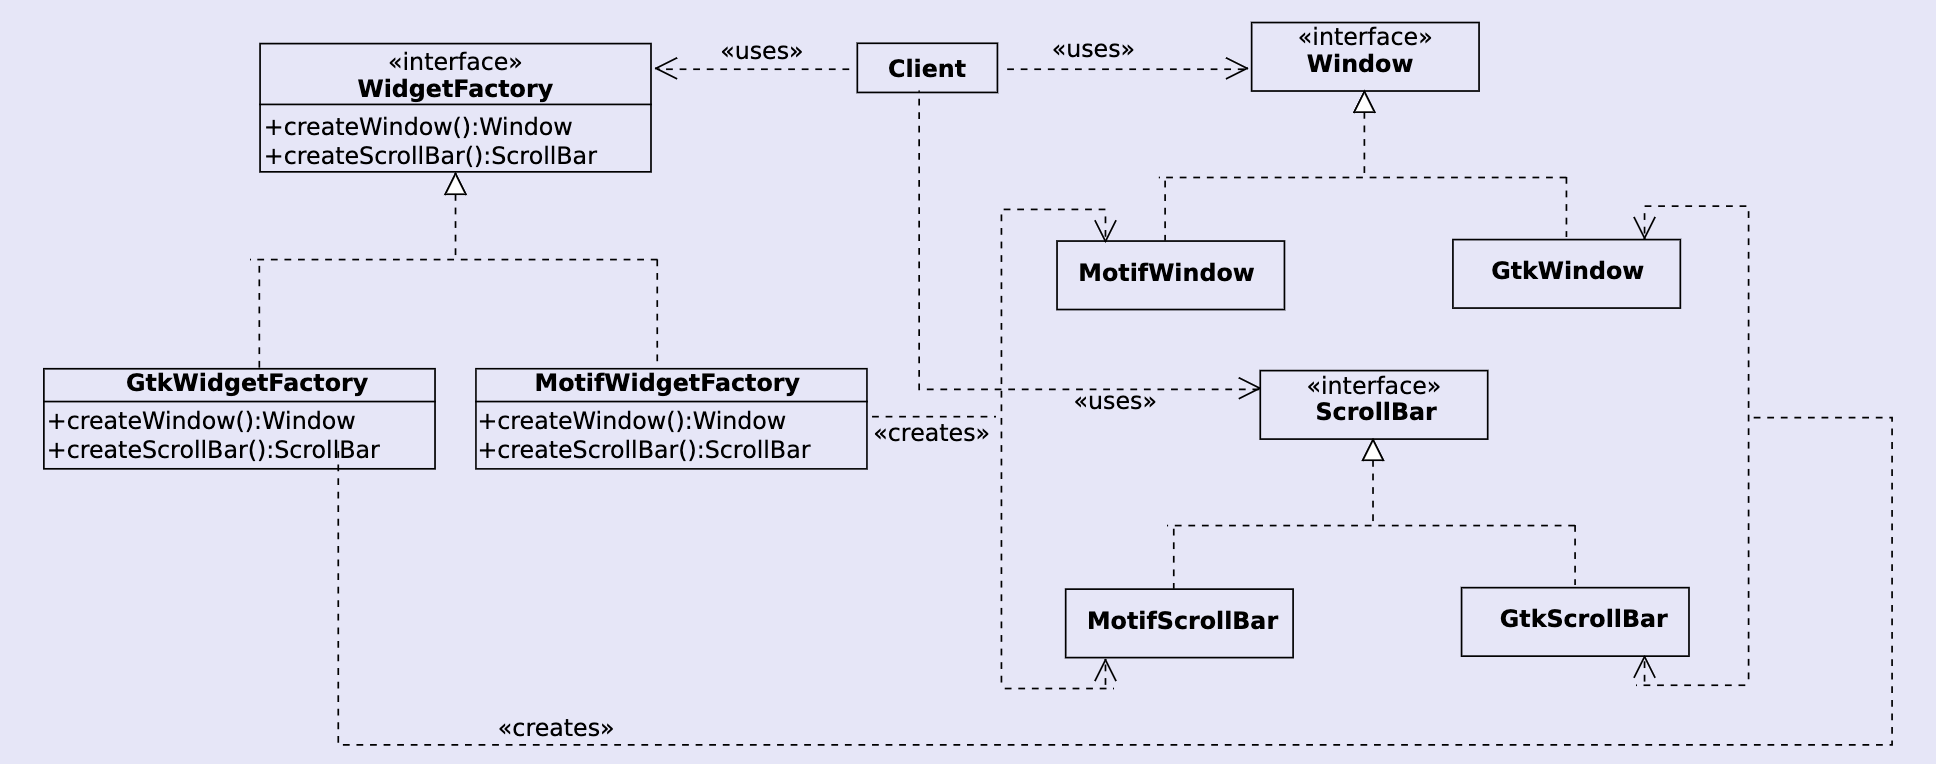
\includegraphics[width=1\linewidth]{assets/pattern/abstract-factory/abstract-factory-esempio.png}
\end{figure}

\paragraph{Soluzione} L’interfaccia WidgetFactory introduce un metodo per la creazione di ciascun tipo di base di widget definito a sua volta da un’oportuna interfaccia. I client invocano i metodi definiti da WidgetFactory per ottenere istanze di widget senza conoscere la classe concreta che utilizzano. Esiste una classe concreta che implementa WidgetFactory per ciascuno dei L\&F considerati.

\begin{figure}[H]
    \centering
    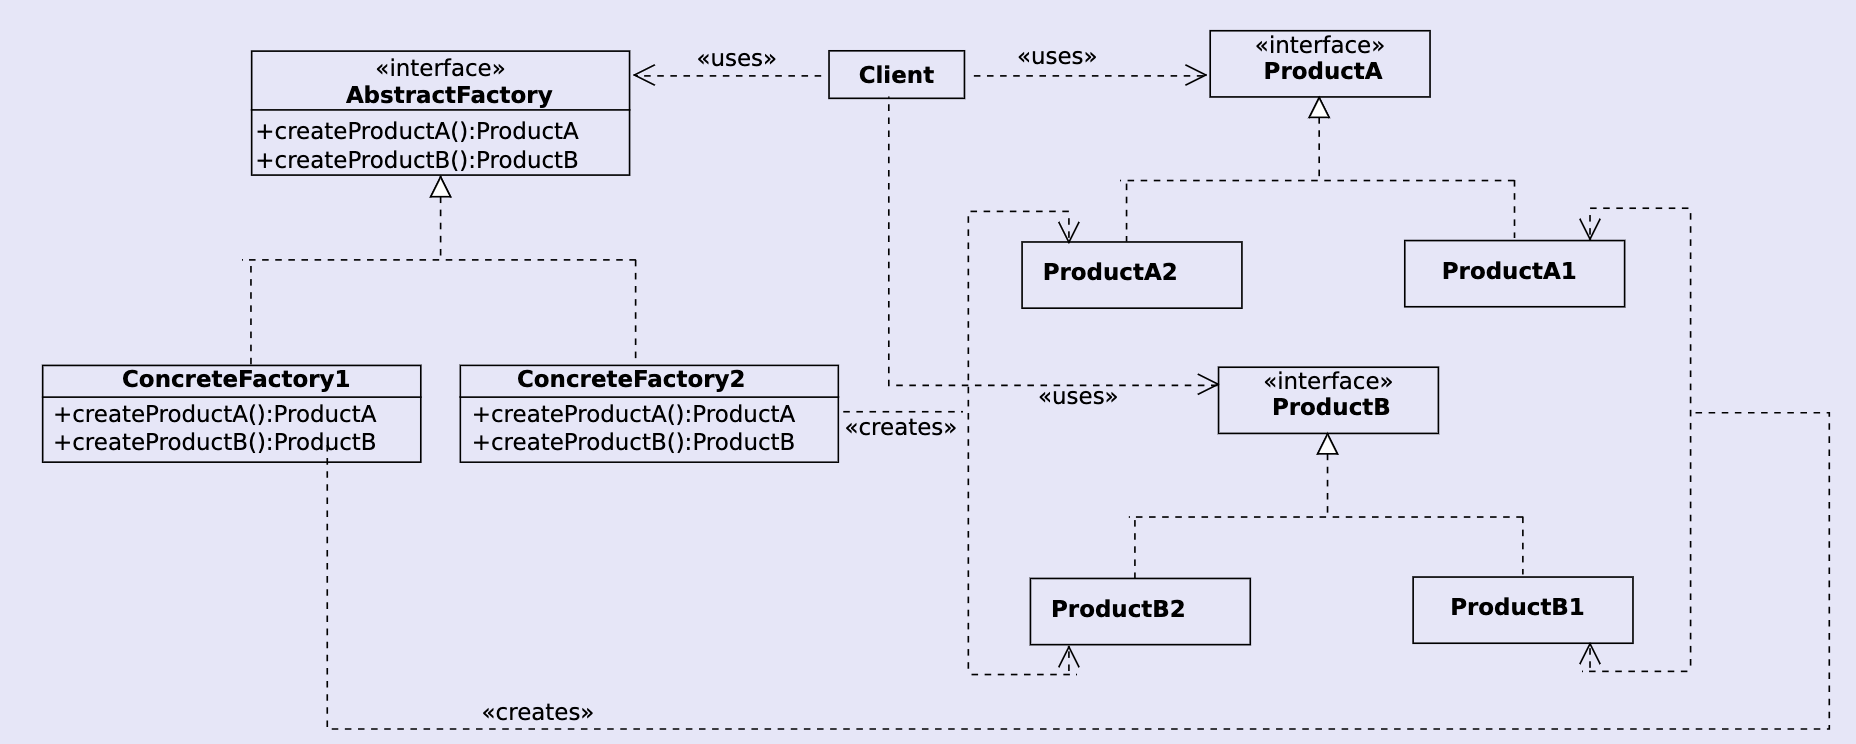
\includegraphics[width=1\linewidth]{assets/pattern/abstract-factory/abstract-factory-struttura.png}
    \caption{Class Diagram del pattern Abstract Factory}
\end{figure}

\paragraph{Struttura e Conseguenze} I partecipanti del pattern sono:
\begin{itemize}
    \item \textbf{AbstractFactory} (WidgetFactory): dichiara un’interfaccia per le operazioni di creazione di oggetti prodotto astratti.
    \item \textbf{ConcreteFactory} (MotifWidgetFactory, GtkWidgetFactory): implementa le operazioni degli oggetti prodotto concreti. 
    \item \textbf{AbstractProduct} (Window, ScrollBar): dichiara un’interfaccia per un tipo di prodotti
    \item \textbf{ConcreteProduct} (MotifWindow, GtkWindow): implementa l’interfaccia Product definendo un oggetto prodotto creato dalla corrispondente factory concreta.
\end{itemize}

Il pattern AbstractFactory consente quindi di isolare le classi concrete (processo di creazione incapsulato nella Factory), cambiare agilmente la famiglia di prodotti utilizzata (cambio di configurazione cambiando il tipo di Factory) e promuovere la coerenza nell'utilizzo dei prodotti.

È bene notare che l'aggiunta del supporto a nuove tipologie di prodotti è difficile in quanto comporta la modifica dell'interfaccia AbstractFactory e, di conseguenza, di tutte le classi che la implementano.

In più è possibile implementare il Factory come Singleton (\ref{singleton})

\begin{figure}[H]
    \centering
    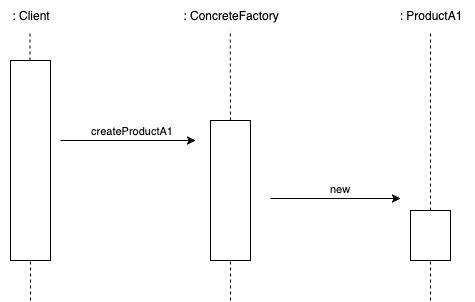
\includegraphics[width=1\linewidth]{assets/pattern/abstract-factory/abstract-factory-sequence.drawio.png}
    \caption{Sequence Diagram del pattern Abstract Factory}
\end{figure}

\newpage
\subsection{Builder}
\label{builder}

\textbf{Scopo}: Creazionale \\
\textbf{Raggio d'azione}: Oggetti

\paragraph{Definizione} Il patter Builder permette di separare la costruzione di un oggetto complesso dalla sua rappresentazione, in modo che lo stesso processo di costruzione possa essere utilizzato per creare rappresentazioni diverse.

\paragraph{Problema} Prendiamo in considerazione un’applicazione capace di leggere documenti in formato RTF che può supportare la conversione in altri formati (ASCII, LaTeX).

\begin{figure}[H]
    \centering
    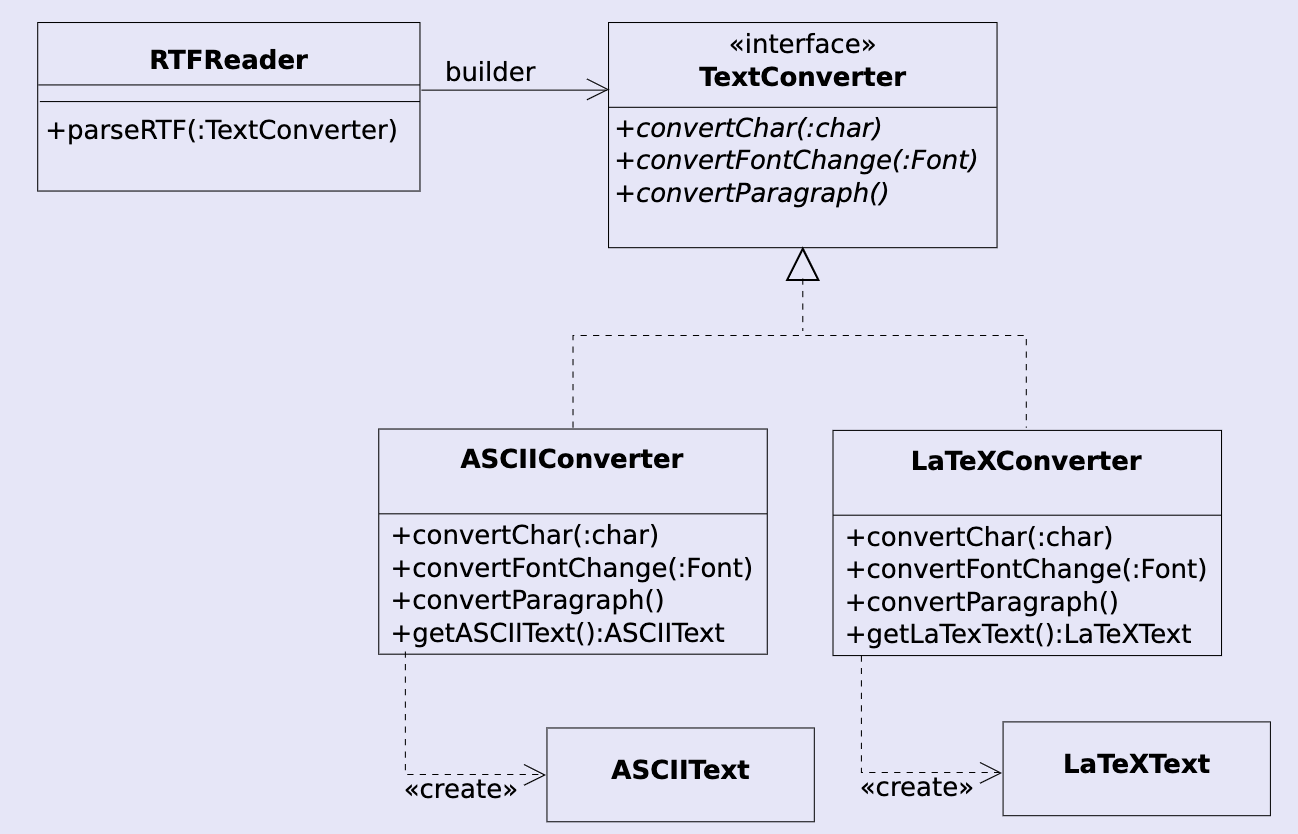
\includegraphics[width=1\linewidth]{assets/pattern/builder/builder-esempio.png}
\end{figure}

\paragraph{Soluzione} Una soluzione consiste nel configurare la classe RTFReader con un oggetto conforme all’interfaccia TextConverter in grado di gestire la conversione in un altro formato. Il documento nel formato di uscita viene costruito man mano che gli elementi del documento RTF sono analizzati.

\begin{figure}[H]
    \centering
    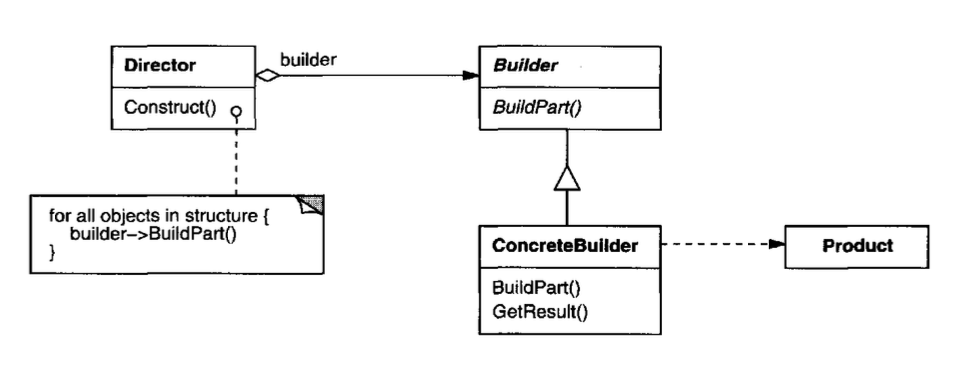
\includegraphics[width=1\linewidth]{assets/pattern/builder/builder-struttura.png}
\end{figure}

\paragraph{Struttura e Conseguenze} Il pattern è composto da:
\begin{itemize}
    \item \textbf{BuilderIF}: specifica l’interfaccia astratta che crea le parti dell’oggetto Product. 
    \item \textbf{ConcreteBuilder}: costruisce e assembla le parti del prodotto implementando l’interfaccia Builder; definisce e tiene traccia della rappresentazione che crea.
    \item \textbf{Director}: costruisce un oggetto utilizzando l’interfaccia Builder.
    \item \textbf{Product}: rappresenta l’oggetto complesso e include le classi che definiscono le parti che lo compongono, includendo le interfacce per assemblare le parti nel risultato finale.
\end{itemize}

Permette quindi di: variare la rappresentazione interna di un prodotto, isolare il codice per la costruzione la rappresentazione e consente di avere maggiore controllo del processo di costruzione.

Risolve allo stesso tempo il problema dei \textbf{costruttori telescopici}, e si propone come alternativa a tecnologie come JavaBeans.

\newpage

\textbf{Esempio Java}

\begin{minted}[
    fontsize=\footnotesize,
    linenos,
]{java}
public class NutritionFacts { 

    private final int servingSize; 
    private final int servings; 
    private final int calories ; 
    private final int fat ; 
    private final int sodium; 
    private final int carbohydrate; 
    
    public static class Builder { 
        // Required parameters 
        private final int servingSize; 
        private final int servings; 
        
        // Optional 
        private int calories = 0; 
        private int fat = 0; 
        private int carbohydrate = 0; 
        private int sodium = 0; 
        
        public Builder( int servingSize, int servings) { 
            this.servingSize = servingSize; 
            this.servings = servings; 
        } 
        
        public Builder calories ( int val ) { 
            calories = val ; return this;
        } 
        
        public Builder fat ( int val ) { 
            fat = val ; 
            return this; 
        } 
        
        public Builder carbohydrate(int val ) {
            carbohydrate = val; 
            return this; 
        } 
        
        public Builder sodium(int val) { 
            sodium = val; 
            return this; 
        } 
        
        public NutritionFacts build () { 
            return new NutritionFacts(this); 
        } 
    }
    
    private NutritionFacts (Builder builder ) { 
        servingSize = builder.servingSize; 
        servings = builder.servings; 
        calories = builder.calories; 
        fat = builder.fat;
        sodium = builder.sodium; 
        carbohydrate = builder.carbohydrate;
    }
}

// Utilizzo:
NutritionFacts cocaCola = new NutritionFacts.Builder(240, 8)
                            .calories(100)
                            .sodium(35)
                            .carbohydrate(27)
                            .build();

\end{minted}

\paragraph{Interazioni} L'utilizzo del pattern consiste nel creare un oggetto Director e configurarlo tramite l'oggetto Builder. Il Director informa il Builder ogni volta che una parte di Product deve essere costruita. Il Builder riceve e gestisce le richieste dal Director e aggiunge le parti al Product. Il client ottiene dal Builder il Product creato.

\begin{figure}[H]
    \centering
    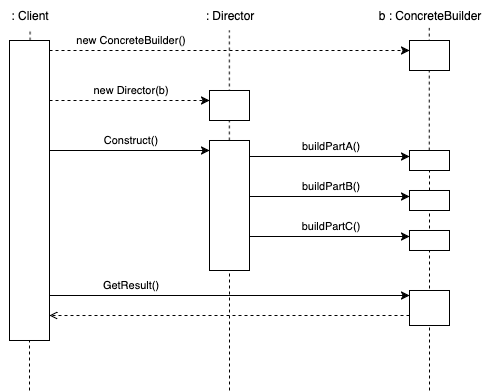
\includegraphics[width=1\linewidth]{assets/pattern/builder/builder-sequence.drawio.png}
\end{figure}

\newpage
\subsection{Factory Method (\textit{o Virtual Constructor})}
\label{factory-method}

\textbf{Scopo}: Creazionale  \\
\textbf{Raggio d'azione}: Classi

\paragraph{Definizione} Definisce un'interfaccia per la creazione di un oggetto, lasciando alle sottoclassi la decisione sulla classe concreta che sarà istanziata. Consente di deferire la creazione di un oggetto alle sottoclassi.

\paragraph{Problema} Si consideri un framework per applicazioni in grado di presentare più documenti agli utenti.

\begin{figure}[H]
    \centering
    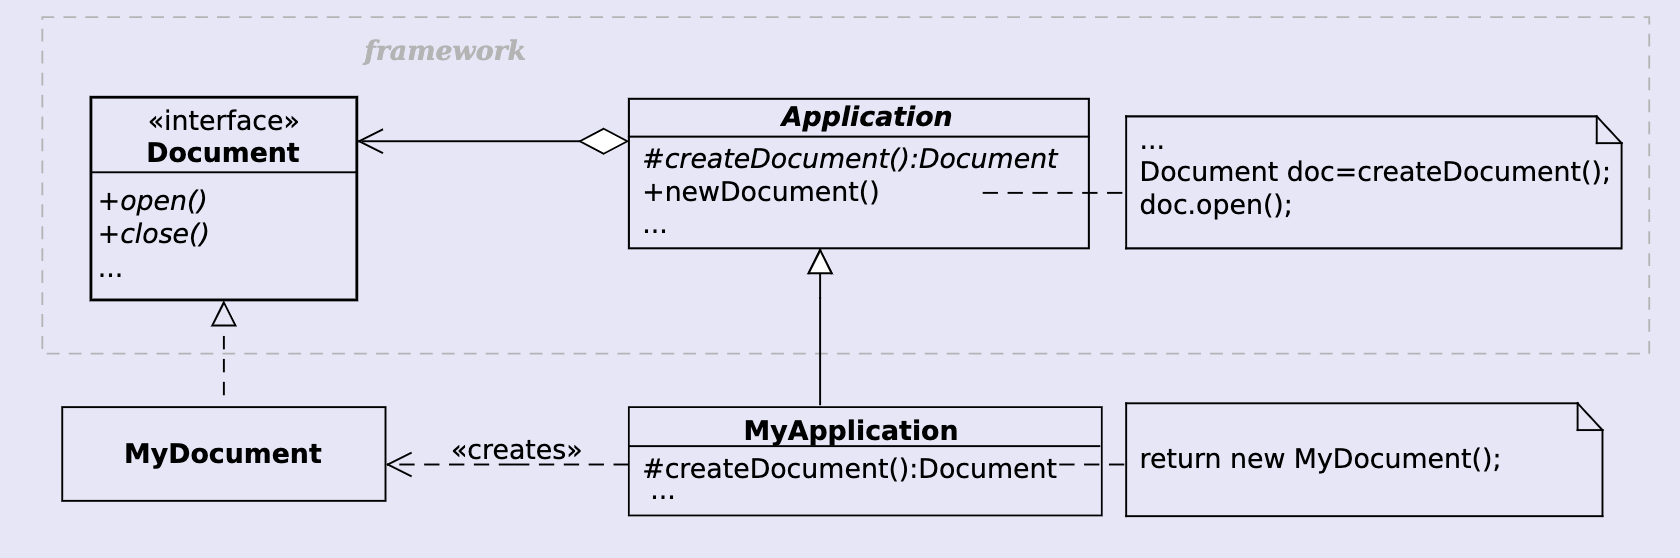
\includegraphics[width=1\linewidth]{assets/pattern/factory-method/factory-method-esempio.png}
\end{figure}

\paragraph{Soluzione} La classe Application è responsabile della gestione di oggetti conformi all’interfaccia Document e della loro creazione. Application sa solo quando dovrà creare un nuovo documento ma non di che tipo né come dovrà farlo. La responsabilità è spostata all’esterno del framework: le sottoclassi di Application devono fornire l’implementazione del metodo factory \textit{createDocument()} in modo da restituire un’istanza della classe appropriata

\paragraph{Struttura e Conseguenze} Il pattern è composto da:
\begin{itemize}
    \item \textbf{Product} (Document): definisce l'interfaccia degli oggetti creati dal metodo factory;
    \item \textbf{ConcreteProduct} (MyDocument): implementa l'interfaccia Product;
    \item \textbf{Creator} (Application): dichiara il metodo factory che restituisce un oggetto di tipo Product. Può invocare \textit{createProduct()} per creare un prodotto;
    \item \textbf{ConcreteCreator} (MyApplication): sovrascrive \textit{createProduct()} in modo da restituire una specifica istanza di ConcreteProduct;
\end{itemize}


\begin{figure}[H]
    \centering
    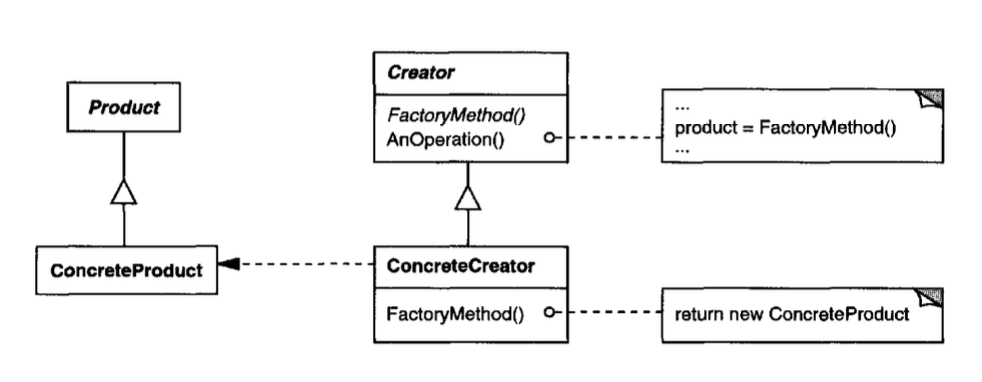
\includegraphics[width=1\linewidth]{assets/pattern/factory-method/factory-method-struttura.png}
    \caption{Class Diagram del pattern Factory Method}
\end{figure}

\begin{itemize}
    \item Elimina la necessità di riferirsi a classi dipendenti dall’applicazione all’interno del codice del framework.
    \item Gli utilizzatori potrebbero essere costretti a definire sottoclassi di Creator per creare un particolare oggetto ConcreteProduct.
    \item Fornisce un punto d’aggancio per le sottoclassi per la produzione di una versione specializzata di un prodotto.
    \item Connette gerarchie di classi parallele. Il metodo factory potrebbe invocato da oggetti diversi dal Creator.
\end{itemize}

\begin{figure}[H]
    \centering
    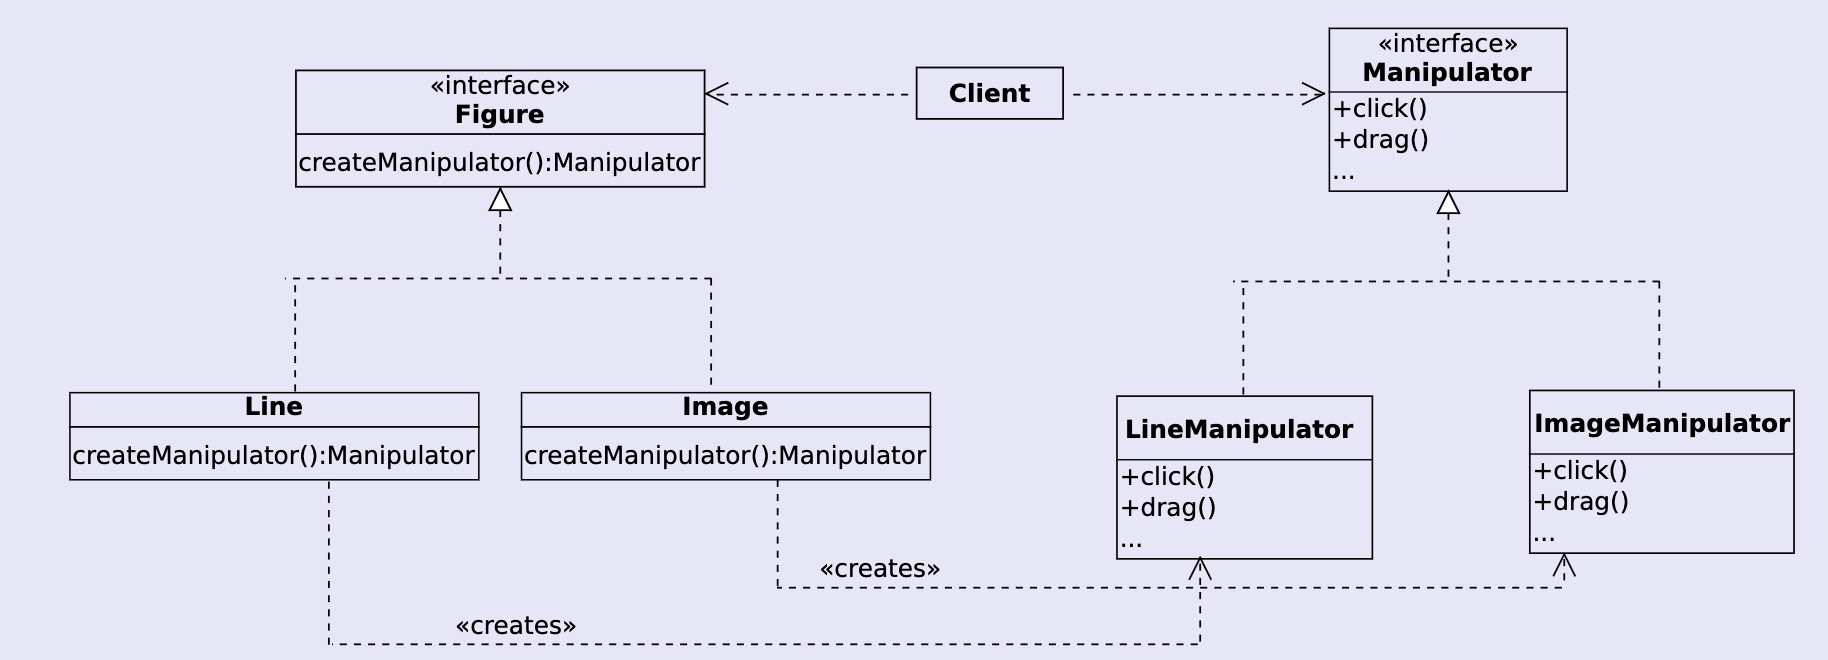
\includegraphics[width=0.8\linewidth]{assets/pattern/factory-method/factory-method-parallelo.png}
    \caption{Gerarchie di classi parallele}
\end{figure}

\begin{figure}[H]
    \centering
    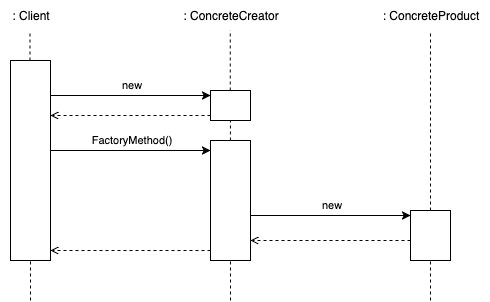
\includegraphics[width=0.8\linewidth]{assets/pattern/factory-method/factory-method-sequence.drawio.png}
    \caption{Sequence Diagram del pattern Factory Method}
\end{figure}

\newpage
\subsection{Prototype}
\label{prototype}

\textbf{Scopo}: Creazionale \\
\textbf{Raggio d'azione}: Oggetti

\paragraph{Definizione} Specifica la tipologia di oggetti da creare utilizzando un'istanza prototipo e creare nuovi oggetti clonando questo prototipo.

\paragraph{Problema} Si pensi ad applicazione che consenta rappresentare degli elementi grafici nel piano cartesiano. L’applicazione potrebbe avere una barra di tasti per effettuare varie operazioni. Un’azione tipica è quella di creare un nuovo oggetto grafico. Per inserire differenti oggetti l’azione da compiere e` identica a parte il tipo di oggetto da creare.

\paragraph{Soluzione} Una soluzione consiste nel configurare l’oggetto responsabile della creazione (il tasto) con un prototipo dell’oggetto da creare.

\begin{figure}[H]
    \centering
    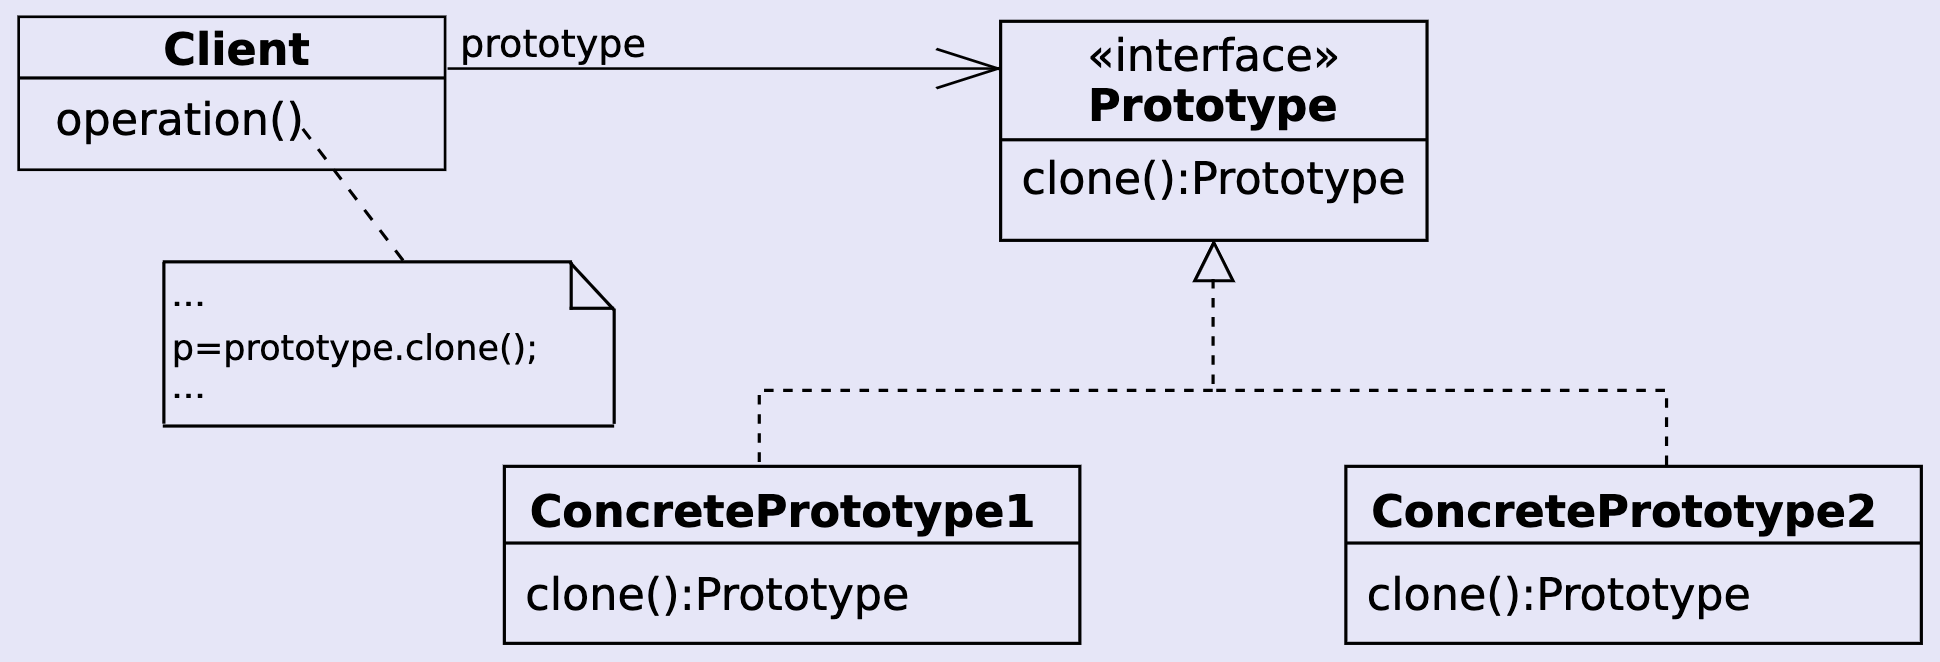
\includegraphics[width=0.75\linewidth]{assets/pattern/prototype/prototype-struttura.png}
    \caption{Class Diagram del pattern Prototype}
\end{figure}

\paragraph{Struttura e Conseguenze} Il pattern è composto da:
\begin{itemize}
    \item \textbf{Prototype}: specifica l'interfaccia che consente la clonazione
    \item \textbf{ConcretePrototype}: implementa l'operazione di clonazione
    \item \textbf{Client}: crea un nuovo oggetto chiedendo ad un prototipo di clonarsi
\end{itemize}

Condivide molte delle conseguenze di Abstract Factory (\ref{abstract-factory}) e Builder (\ref{builder}): nasconde le classi dei prodotti concreti, riducendo il numero di classi che devono essere note al client. In più:
\begin{itemize}
    \item Consente di aggiungere e rimuovere prodotti durante l’esecuzione;
    \item Consente la specifica di nuovi oggetti variando i valori;
    \item Consente la specifica di nuovi oggetti variando la struttura;
    \item Riduce il numero di sottoclassi
    \item Obbliga l'implementazione dell’operazione \textit{clone()}
\end{itemize}

\textbf{In Java}
Utilizzo dell'interfaccia \textit{Cloneable}, è possibile clonare oggetti in modo superficiale (shallow copy) o in maniera profonda (deep copy) ridefinendo il metodo clone().

\begin{minted}[
    fontsize=\footnotesize,
    linenos,
]{java}
// Shallow copy
public class Point2D implements Cloneable {
    private double x; 
    private double y;
    
    @Override public Point2D clone() { 
        try { 
            Point2D clone = (Point2D) super.clone(); 
            return clone;
        } catch (CloneNotSupportedException e) {
            throw new Error(e);
        } 
    } 
}
\end{minted}

\newpage

\begin{minted}[
    fontsize=\footnotesize,
    linenos,
]{java}

// Deep copy
public abstract class PolinomioAstratto implements Polinomio, Cloneable { 
    protected abstract PolinomioAstratto getPrototype(); 

    @Override public Polinomio add(Polinomio p) { 
        // crea un nuovo polinomio 
        Polinomio somma = getPrototype().clone(); 

        // aggiunge ciascun monomio di this al polinomio somma 
        for (Monomio m : this) somma.add(m); 
        
        // aggiunge ciascun monomio di p al polinomio somma 
        for (Monomio m : p) somma.add(m); 
        
        return somma; 
    } 
    
    @Override public PolinomioAstratto clone() { 
        try { 
            return (PolinomioAstratto) super.clone(); 
        } catch (CloneNotSupportedException e) { 
            throw new Error(e); 
        }
    }
}

public class PolinomioLL extends PolinomioAstratto { 
    private static PolinomioLL prototype; 
    private LinkedList<Monomio> monomi = new LinkedList<>(); 
    
    @Override protected synchronized PolinomioLL getPrototype() { 
        if ( prototype==null ) prototype = new PolinomioLL(); 
        return prototype;
    } 
    
    @Override public PolinomioLL clone() {
        PolinomioLL p = (PolinomioLL) super.clone();
        p.monomi = new LinkedList<Monomio>(); 
        for (Monomio m : this) p.monomi.add(m); 
        return p;
    }
}

\end{minted}

\newpage
\subsection{Singleton}
\label{singleton}

\textbf{Scopo}: Creazionale \\
\textbf{Raggio d'azione}: Oggetti

\paragraph{Definizione} Il pattern Singleton assicura che un classe abbia una sola istanza e fornisca un solo punto di accesso globale a tale istanza.

\paragraph{Problema} In un sistema potrebbero esistere più stampanti, ma potrebbe essere presente soltanto una coda di stampa. In un sistema operativo dovrebbe essere presente solo un file system e un solo window manager

\paragraph{Soluzione} Per assicurare che una classe abbia una sola istanza e che tale istanza sia facilmente accessibile per gli utilizzatori si può fare in modo che la classe stessa abbia la responsabilità di creare le proprie istanze. La classe può assicurare che nessun’altra istanza possa essere creata e può fornire un modo semplice per accedere all’istanza.

\begin{figure}[H]
    \centering
    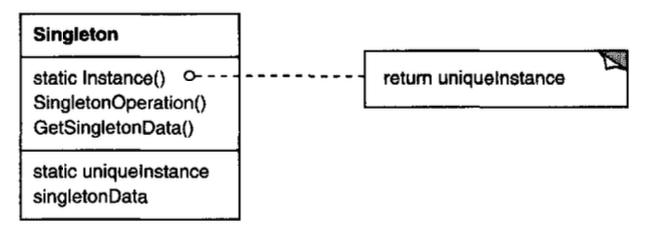
\includegraphics[width=0.4\linewidth]{assets/pattern/singleton/singleton-struttura.png}
    \caption{Class Diagram del pattern Singleton}
\end{figure}

\paragraph{Struttura e Conseguenze} Il pattern risulta essere applicabile in due casi in particolare:
\begin{itemize}
    \item Quando deve esistere esattamente un’istanza di una classe resa accessibile ai client attraverso un punto di accesso noto a tutti gli utilizzatori.
    \item Quando l’unica istanza deve poter essere estesa attraverso la definizione di sottoclassi ed i client devono essere in grado di utilizzare le istanze estese senza dover modificare il proprio codice.
\end{itemize}

\textbf{Java}

\begin{minted}[
    fontsize=\footnotesize,
    linenos,
]{java}
public final class Singleton { 
    private static Singleton INSTANCE = null; 
    
    private Singleton(){} 
    
    public static synchronized Singleton getInstance() { 
        if (INSTANCE == null) { 
            INSTANCE=new Singleton(); 
        } 
        return INSTANCE; 
    } 
}
\end{minted}

\newpage

\section{Strutturali}

I pattern strutturali si occupano di come classi e oggetti sono composti per formare strutture più grandi. 
\begin{itemize}
    \item \textbf{Class Structural}: usano l'ereditarietà per definire interfacce o implementazioni;
    \item \textbf{Object Structural}: descrivono modi per comporre oggetti per realizzare nuove funzionalità
\end{itemize}

È bene sottolineare che alcuni pattern fanno utilizzo di ereditarietà multipla, non sempre applicabile in linguaggi come Java, che permettono di implementare molteplici interfacce, ma estendere una sola classe (astratta o concreta).

\subsection{Adapter (\textit{o Wrapper})}
\label{adapter}

\textbf{Scopo}: Strutturale \\
\textbf{Raggio d'azione}: Classi, Oggetti

\paragraph{Definizione} Permette di convertire l'interfaccia di una classe in un'altra interfaccia richiesta dal client.Consente a classi diverse di cooperare quando ciò non sarebbe possibile a causa di interfacce incompatibili.

\paragraph{Motivazione} A volte una classe preesistente, progettata per essere riutilizzata, non può essere riusata perché incompatibile con l'interfaccia richiesta dall'applicazione. Nell’esempio, la classe XXXTriangle non può essere riusata dove ci si aspetta l’interfaccia Figure2D perché non è compatibile con essa.

\begin{multicols}{2}
\begin{figure}[H]
    \centering
    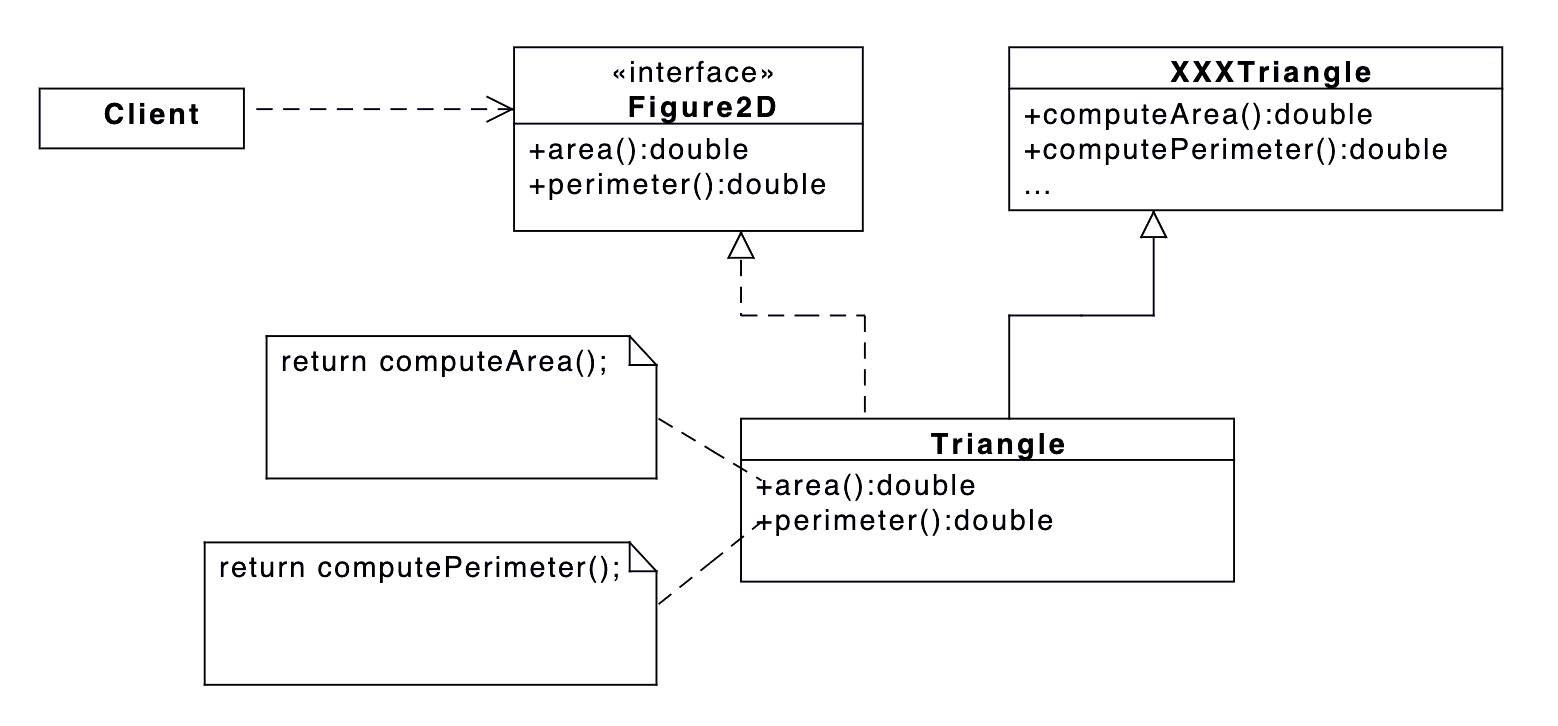
\includegraphics[width=1\linewidth]{assets/pattern/adapter/adapter-esempio-class.png}
    \caption{Esempio di Class Adapter}
\end{figure}
\columnbreak
\begin{figure}[H]
    \centering
    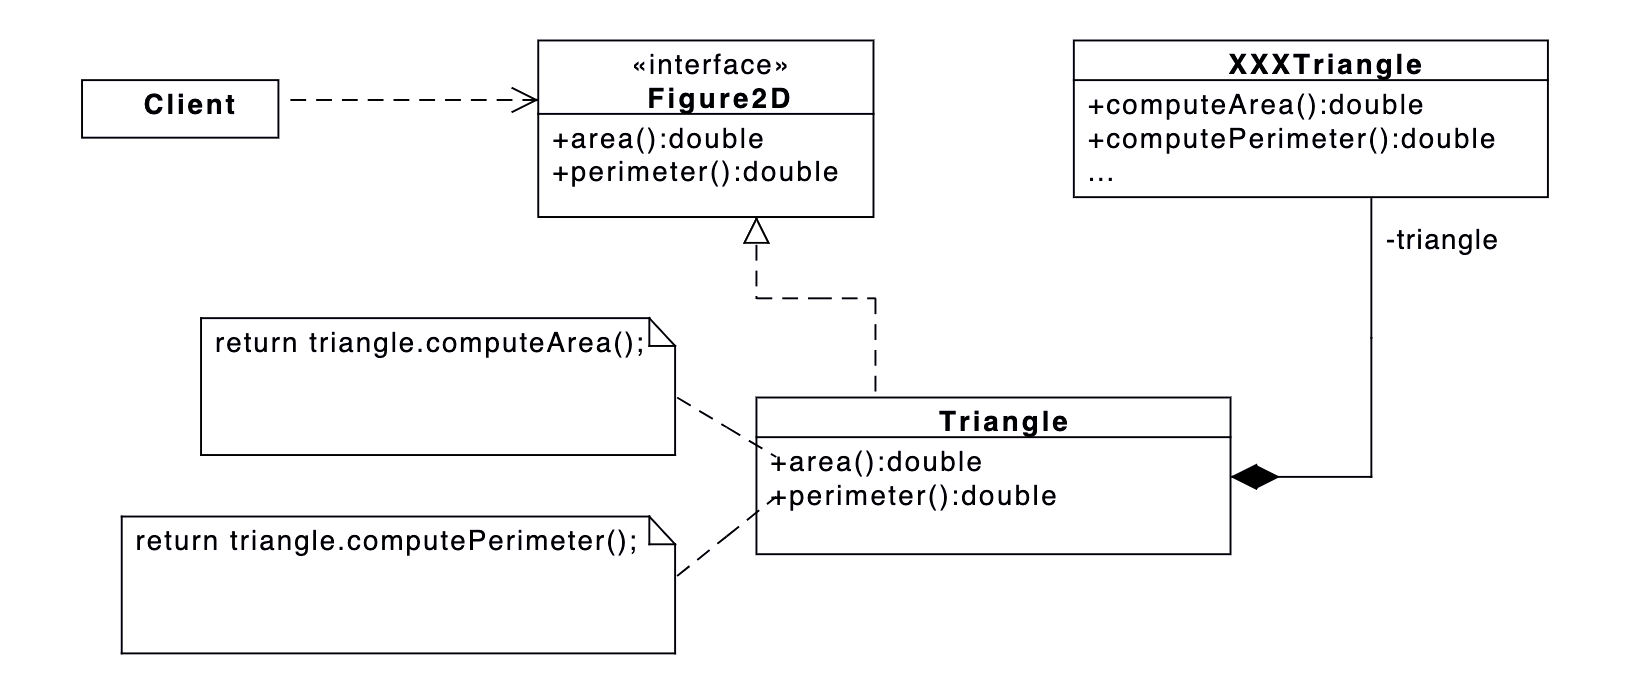
\includegraphics[width=1\linewidth]{assets/pattern/adapter/adapter-esempio-object.png}
    \caption{Esempio di Object Adapter}
\end{figure}
\end{multicols}

Pensare di modificare XXXTriangle per renderla conforme a Figure2D non è una buona soluzione (si legherebbe al contesto specifico e il codice sorgente potrebbe non essere disponibile).

Si introduce una classe Triangle che sia al contempo erede di entrabe XXXTriangle e Figure2D. L'implementazione dei metodi di Figure2D sfrutta quelli di XXXTriangle.

È possibile introdurre la classe Triangle anche di modo che faccia riferimento ad un oggetto (istanza di XXXTriangle) e vada ad implementare l'interfaccia Figure2D delegando l'esecuzione all'oggetto incapsulato.

\begin{figure}[H]
    \centering
    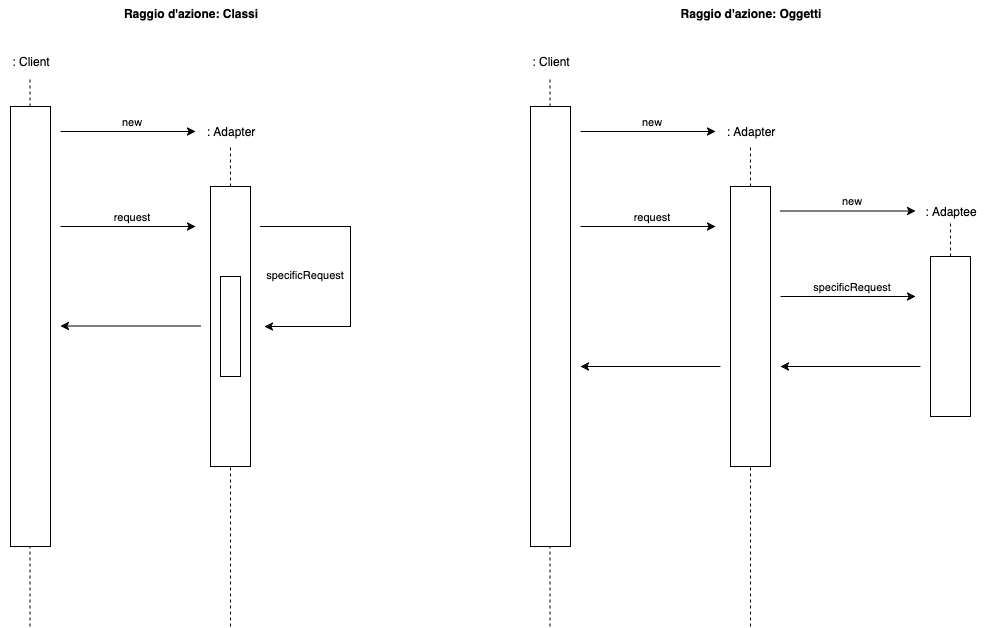
\includegraphics[width=0.75\linewidth]{assets/pattern/adapter/adapter-sequence.drawio.png}
    \caption{Sequence diagram raggio d'azione}
\end{figure}

\paragraph{Applicabilità} È consigliabile utilizzare il pattern Adapter quando:
\begin{itemize}
    \item Si vuole utilizzare una classe esistente e la sua interfaccia non è compatibile con quella che serve;
    \item Si vuole creare una classe riusabile che coopera con classi non correlate o non conosciute;
    \item Si vogliono usare varie sottoclassi esistenti, ma non sarebbe pratico adattare le loro interfacce tramite ereditarietà (solo per object);
\end{itemize}

\paragraph{Struttura} Il pattern è composto dai seguenti partecipanti:
\begin{itemize}
    \item \textbf{Target} (Figure2D): definisce l'interfaccia specifica del dominio utilizzata dal client
    \item \textbf{Client}: collabora con oggetti compatibili con l'intefaccia Target
    \item \textbf{Adaptee} (XXXTriangle): individua un'interfaccia che deve essere adattata.
    \item \textbf{Adapter} (Triangle): adatta l'interfaccia Adaptee al'interfaccia Target
\end{itemize}

I client invocano le operazioni su un'istanza di Adapter, il quale invoca operazioni di Adaptee per soddisfare la richiesta

\begin{figure}[H]
    \centering
    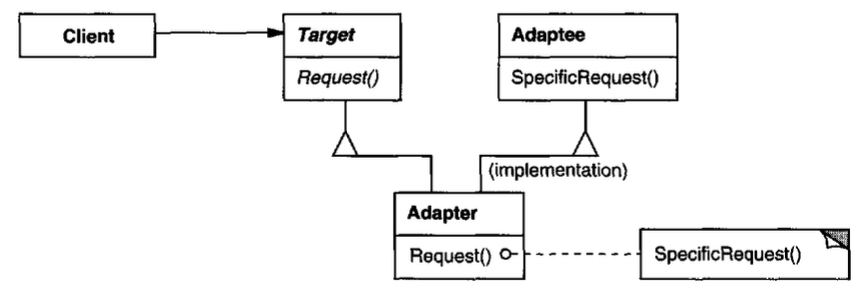
\includegraphics[width=0.75\linewidth]{assets/pattern/adapter/adapter-struttura-class.png}
    \caption{Class Diagram di Adapter (Class)}
\end{figure}

\begin{figure}[H]
    \centering
    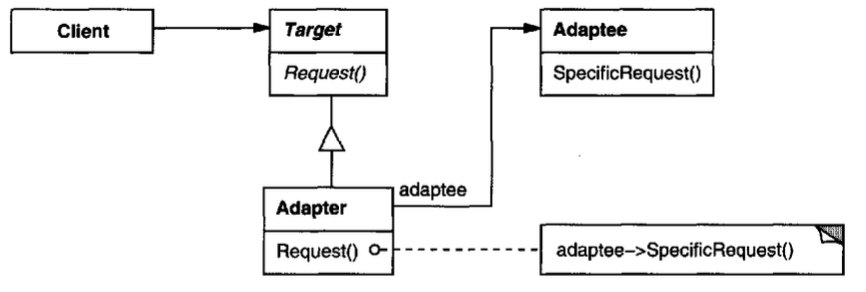
\includegraphics[width=0.75\linewidth]{assets/pattern/adapter/adapter-struttura-object.png}
    \caption{Class Diagram di Adapter (Object)}
\end{figure}

\paragraph{Conseguenze} Il pattern Builder consente quindi di:
\begin{itemize}
    \item Scegliere lo spettro di operazioni da supportare (o wrappare);
    \item Supportare i \textbf{pluggable adapter}: classi che supportano l'adattamento di interfaccia
    \item Usare i \textbf{two-way adapters}: permettono all'Adapter di supportare operazioni dell'Adaptee e viceversa.
\end{itemize}

\textbf{Class Adapter}
\begin{itemize}
    \item Adatta l'interfaccia Adaptee all'interfaccia Target basandosi su una classe concreta.
    \item Non può essere utilizzata se Adaptee è astratta oppure è un'interfaccia.
    \item Consente ad Adapter di sovrascrivere parte del comportamento di Adaptee essendo una sua sottoclasse
    \item Non occorrono ulteriori indirezioni per raggiungere l'oggetto adattato
\end{itemize}

\textbf{Object Adapter}
\begin{itemize}
    \item Permette ad un singolo Adapter di operare con Adaptee e le sue sottoclassi, se esistono. Può in tal caso aggiungere funzionalità a tutti gli Adaptee
    \item Rende difficile sovrascrivere il comportamento di Adaptee non essendo una sua sottoclasse
    \item Aggiunge un livello di indirezione per raggiungere l'oggetto adattato.
\end{itemize}

\newpage
\subsection{Bridge (\textit{o Handle, Body})}
\label{bridge}

\textbf{Scopo}: Strutturale \\
\textbf{Raggio d'azione}: Oggetti

\paragraph{Definizione} Disaccoppia un’astrazione dalla sua implementazione in modo che le due possano variare indipendentemente l’una dall’altra. È spesso utilizzato all’inizio di un progetto per consentire ad astrazioni ed implementazioni di variare in modo indipendente.

\paragraph{Problema} Quando un’astrazione può avere una tra più implementazioni possibili, in genere si risolve il problema ricorrendo all’ereditarietà. L’astrazione viene definita da un’interfaccia o da una classe astratta e le sottoclassi concrete la implementano in modi differenti. Tale approccio non è flessibile poichè l’ereditarietà lega un’implementazione ad un’astrazione in modo permanente. Ciò rende difficile modificare, estendere e riusare astrazioni ed implementazioni in modo indipendente.

\paragraph{Esempio} Si supponga di volere scrivere un toolkit per la realizzazione di interfacce grafiche. Sicuramente ci sarebbe il bisogno di un’astrazione Window per rappresentare una finestra. Si vuole far in modo che il toolkit funzioni con diversi gestori grafici come ad esempio X Windows o IBM Presentation Manager.

\begin{figure}[H]
    \centering
    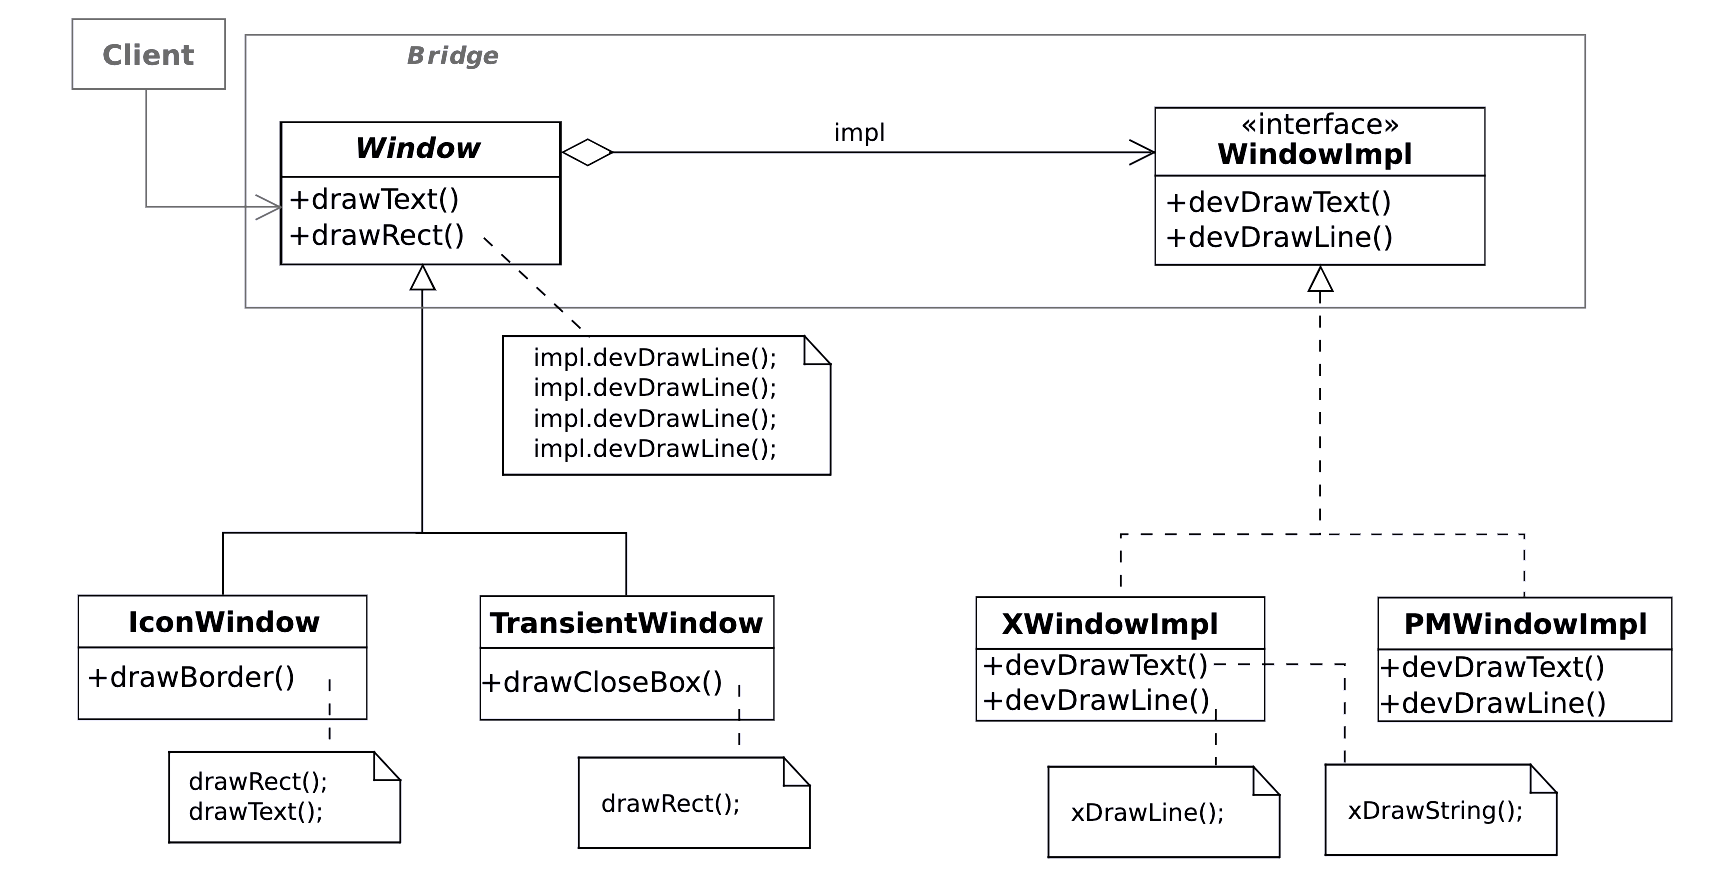
\includegraphics[width=1\linewidth]{assets/pattern/bridge/bridge-esempio.png}
\end{figure}

Si può fare ricorso all’ereditarietà rendendo Window una classe astratta (o un’interfaccia) ed introducendo due sottoclassi XWindow e PMWindow per fornire due implementazioni dell’astrazione. Tale approccio ha due difetti principali:

\begin{itemize}
    \item È scomodo estendere l’astrazione Window per supportare tipologie diverse di finestre o nuove piattaforme. Se ad esempio si volesse introdurre una specializzazione IconWindow per le icone, occorrerebbe anche introdurre due sottoclassi XIconWindow e PMIconWindow per le due piattaforme.
    \item Il codice del client diventa dipendente dalla piattaforma utilizzata. Ogni volta che occorre creare una finestra occorre istanziare una specifica classe concreta.
\end{itemize}

\paragraph{Soluzione} Il pattern Bridge risolve questi problemi introducendo due gerarchie separate: una per le astrazioni (Window,IconWindow, TransientWindow) ed una (con radice, WindowImpl) per le diverse implementazioni dipendenti dalla piattaforma. I metodi di Window sono tutti implementati in termini dei metodi di WindowImpl. La relazione tra Window e WindowImpl è detta bridge in quanto funge da ponte tra un’astrazione ed una implementazione consentendo ad entrambe di variare indipendentemente.

\begin{figure}[H]
    \centering
    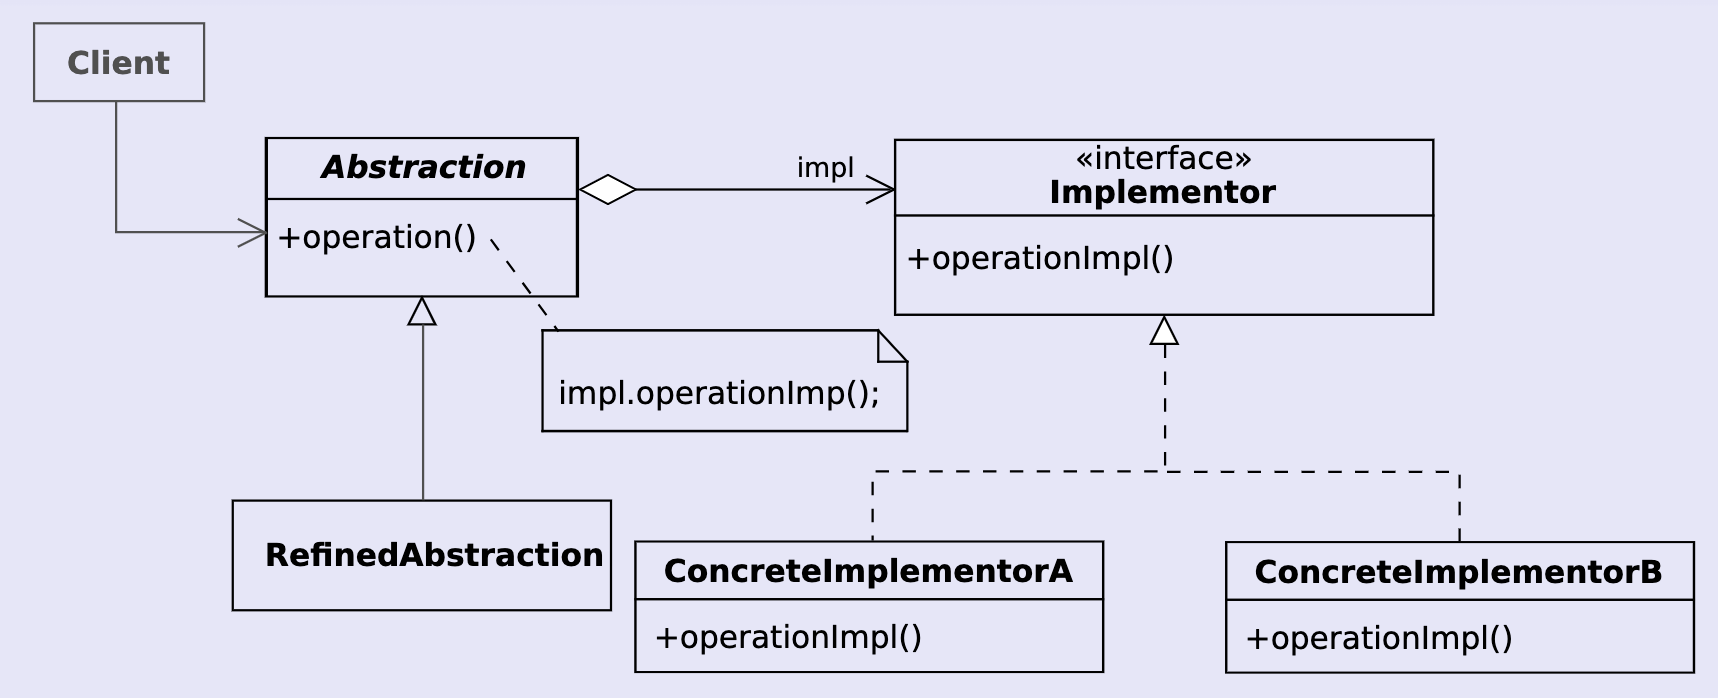
\includegraphics[width=1\linewidth]{assets/pattern/bridge/bridge-struttura.png}
\end{figure}

\paragraph{Struttura e Conseguenze} I partecipanti del pattern Bridge sono:
\begin{itemize}
    \item \textbf{Abstraction}: specifica l’interfaccia dell’astrazione. Mantiene un riferimento ad un oggetto di tipo Implementor;
    \item \textbf{RefinedAbstraction}: Estende l’interfaccia definita da Abstraction;
    \item \textbf{Implementor}: definisce l’interfaccia per le classi che implementano l’astrazione. Non deve corrispondere esattamente all’interfaccia di Abstraction: Implementor fornisce le operazioni base, mentre Abstraction definisce operazioni di più alto livello implementate sfruttando quelle di base;
    \item \textbf{ConcreteImplementor}: definisce un’implementazione concreta dell’interfaccia Implementor.
\end{itemize}

L'utilizzo del pattern permette quindi maggiore \textbf{disaccoppiamento} tra interfaccia ed implementazione, maggiore \textbf{estensibilità} e mascheramento dei dettagli implementativi al client.

È possibile utilizzare Abstract Factory (\ref{abstract-factory}) per creare e configurare un particolare Bridge.

Il pattern Adapter (\ref{adapter}) permette di far cooperare classi non correlate a valle della loro implementazione.

\newpage
\subsection{Composite}
\label{composite}

\textbf{Scopo}:  \\
\textbf{Raggio d'azione}: 

\paragraph{Definizione}

\paragraph{Problema}

\paragraph{Soluzione} 

\paragraph{Struttura e Conseguenze} 

\newpage
\subsection{Decorator}
\label{decorator}

\textbf{Scopo}: Strutturale \\
\textbf{Raggio d'azione}: Oggetti

\paragraph{Definizione} Il pattern decorator permetter di aggiungere dinamicamente responsabilità ad un oggetto. Fornisce un'alternativa flessibile all'uso dell'ereditarietà come strumento per l'estensione delle funzionalità.

\paragraph{Problema} Talvolta è necessario aggiungere responsabilità ad un singolo oggetto e non ad un intera classe.

Esempio: Libreria per la realizzazione di interfacce utente deve permettere di aggiungere bordi o altri elementi a ciascun componente grafico.

Ricorrere all'ereditarietà complicherebbe la cosa, andrebbero create sottoclassi per ogni componente aggiuntivo, in più renderebbe difficile comporre più estensioni di comportamento.

\paragraph{Soluzione} Racchiudere il componente da decorare dentro un altro che sarà responsabile di disegnare il bordo o aggiungere altri componenti visivi. L'oggetto contenitore è detto \textit{decoratore} ed ha la stessa interfaccia dell'oggetto decorato così da poter essere trasparente al client. È possibile che svolga azioni aggiuntive prima o dopo aver trasferito la richiesta all'oggetto decorato.

\begin{figure}[H]
    \centering
    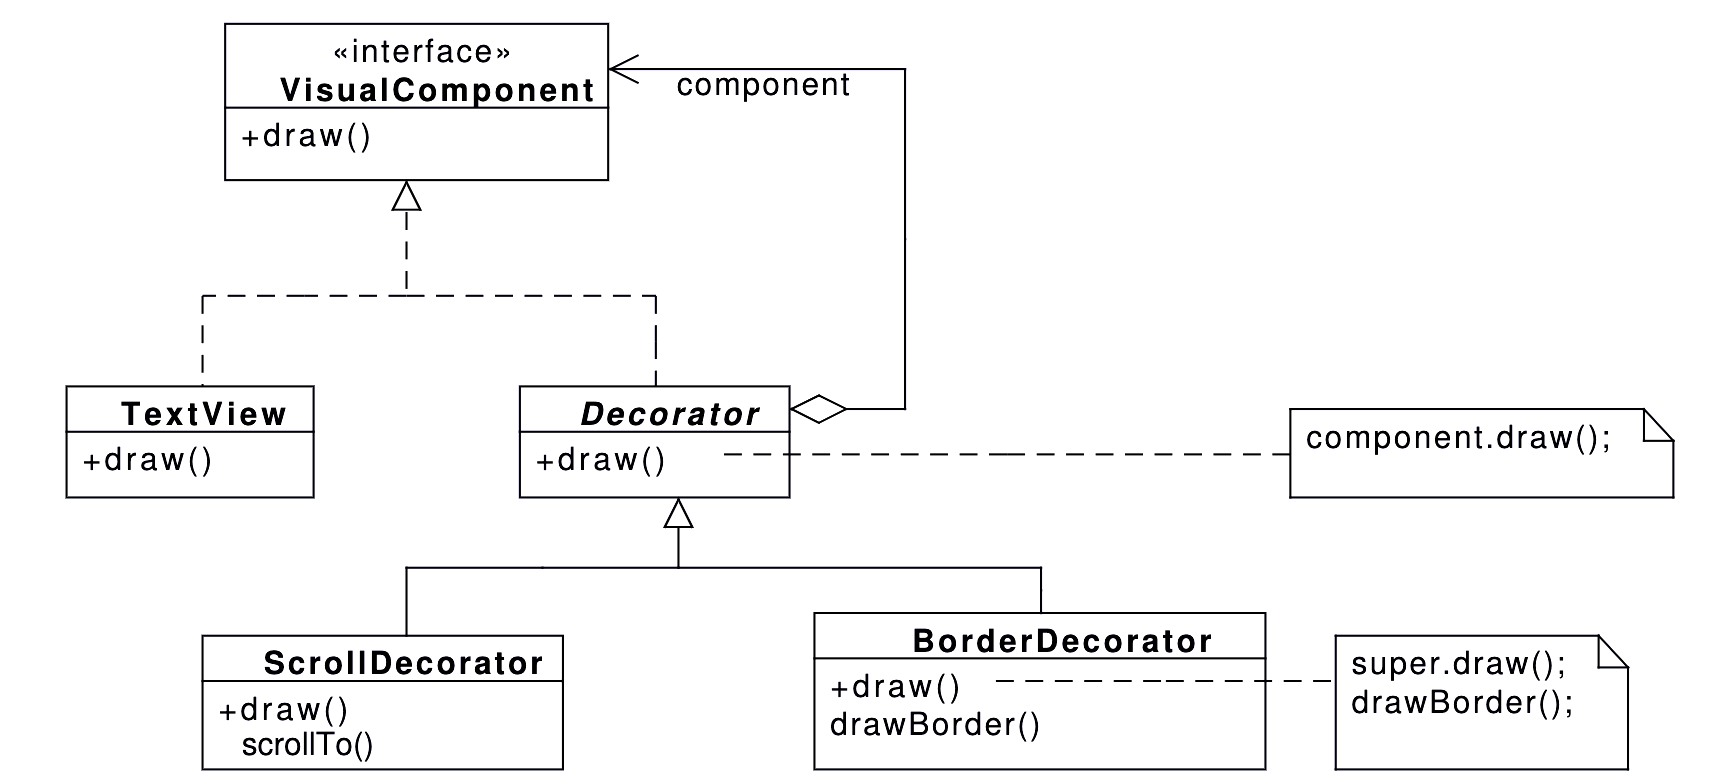
\includegraphics[width=1\linewidth]{assets/pattern/decorator/decorator-esempio.png}
    \caption{Esempio di utilizzo del pattern}
\end{figure}

Nell'esempio l'interfaccia VisualComponent definisce il tipo generico di componenti visuali. La classe TextView consente di visualizzare del testo in una finestra. La classe astratta Decorator inoltra semplicemente le richieste al componente incapsulato. BorderDecorator e ScrollDecorator consentono rispettivamente di aggiungere bordi e barre di scorrimento.

\paragraph{Struttura e Conseguenze} Il pattern è composto dai seguenti partecipanti:
\begin{itemize}
    \item \textbf{ServiceIF} (VisualComponent): definisce l'interfaccia comune per gli oggetti ai quali possono essere aggiunte nuove responsabilità dinamicamente.
    \item \textbf{ConcreteService} (TextView): definisce un oggetto al quale possono essere aggiunte ulteriori responsabilità
    \item \textbf{Decorator}: mantiene un riferimento ad un oggetto di tipo ServiceIF e, al contempo implementa l'interfaccia ServiceIF.
    \item \textbf{ConcreteDecorator} (ScrollDecorator, BorderDecorator): aggiunge responsabilità al componente
\end{itemize}


\begin{figure}[H]
    \centering
    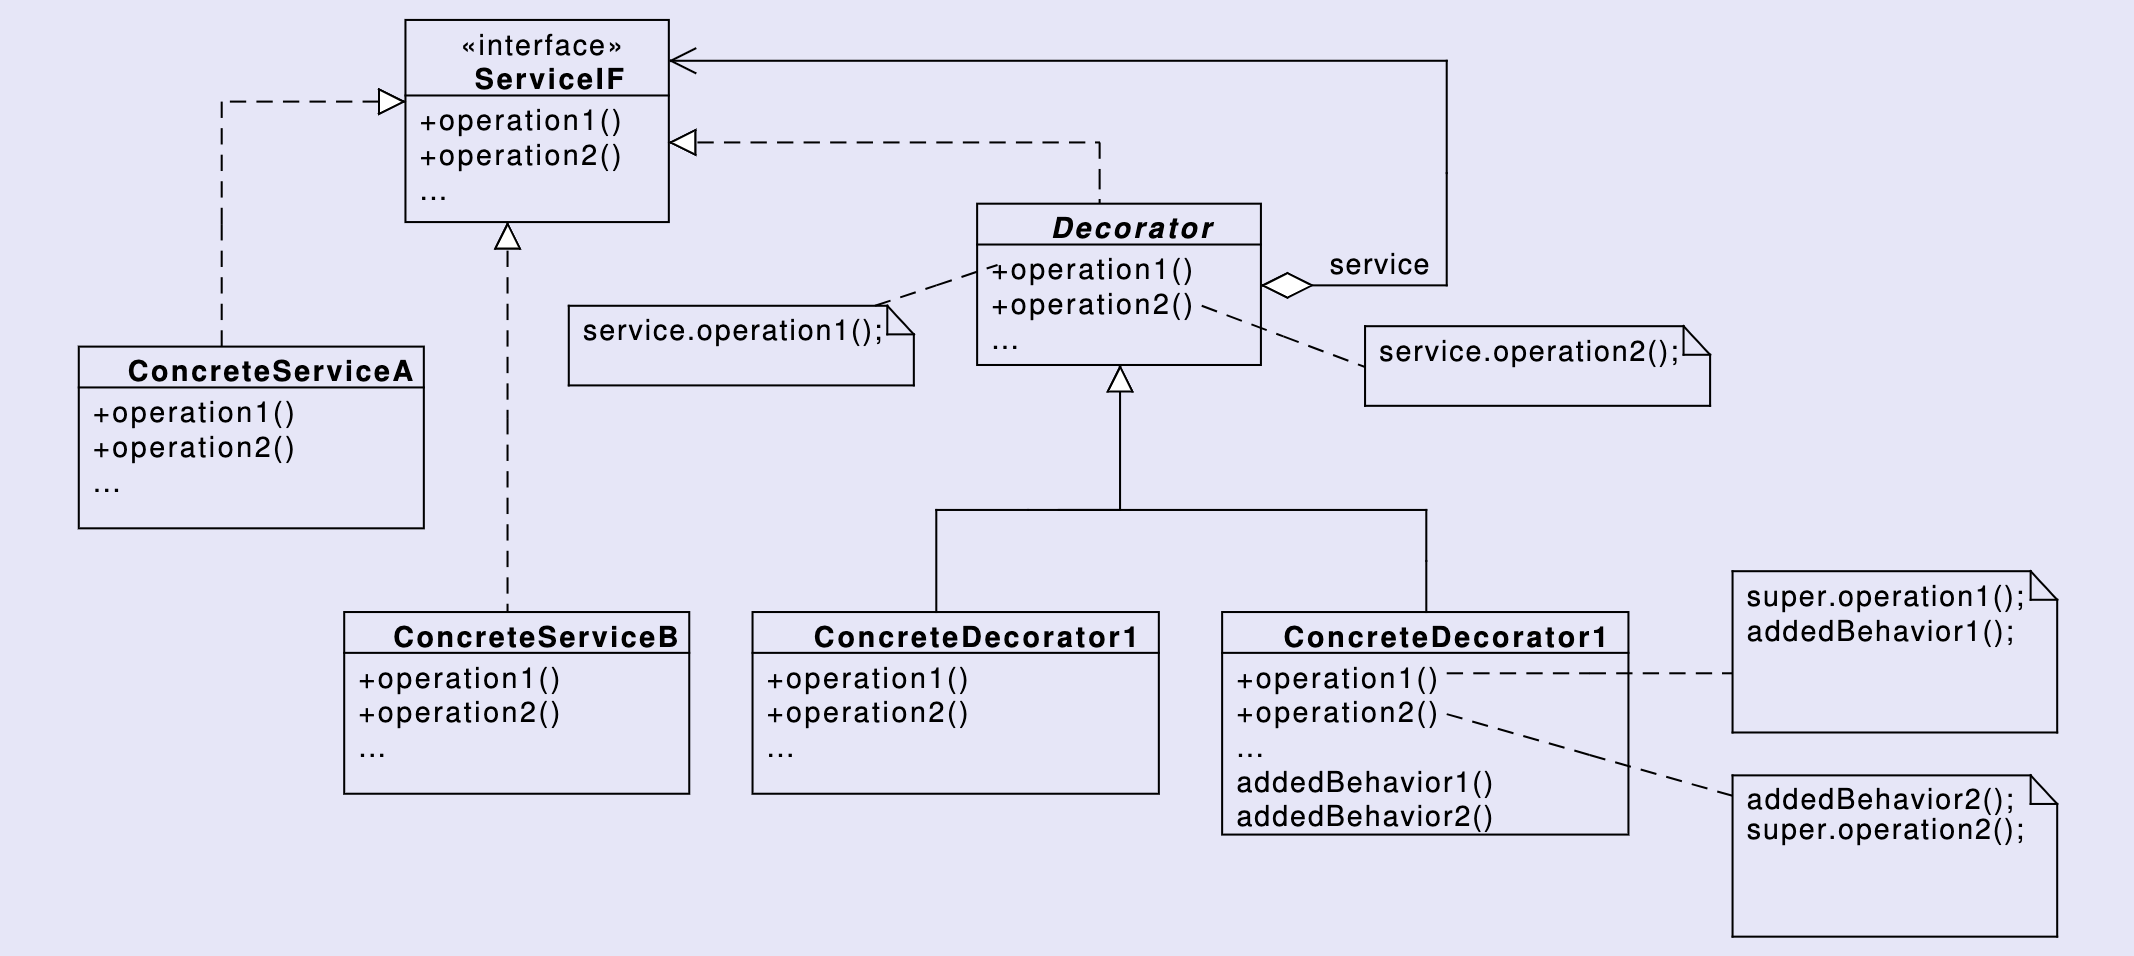
\includegraphics[width=1\linewidth]{assets/pattern/decorator/decorator-struttura.png}
    \caption{Class Diagram del pattern Decorator}
\end{figure}

\begin{itemize}
    \item Maggiore flessibilità rispetto all'ereditarietà;
    \item Differenti combinazioni di oggetti attraverso l'utilizzo di diversi decoratori;
    \item L'uso nei progetti porta a sistemi composti di molti oggetti simili interconnessi, facile da interpretare dal progettista, meno da esterni;
    \item Decoratore e oggetto decorato sono uguali in termini di comportamento ma differiscono in termini di identità
    \item Bisogna porre attenzione in come si compongono i decoratori, per esempio evitare dipendenze circolari.
\end{itemize}

\begin{figure}[H]
    \centering
    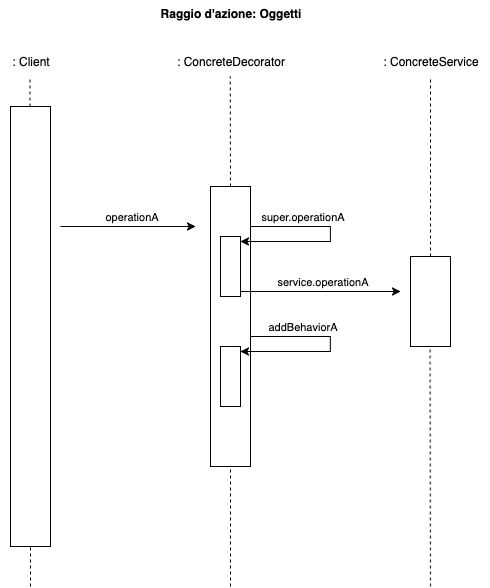
\includegraphics[width=1\linewidth]{assets/pattern/decorator/decorator-sequence.drawio.png}
    \caption{Sequence Diagram del pattern Decorator}
\end{figure}


\newpage
\subsection{Facade}


\textbf{Scopo}:  \\
\textbf{Raggio d'azione}: 

\paragraph{Definizione}

\paragraph{Problema}

\paragraph{Soluzione} 

\paragraph{Struttura e Conseguenze} 

\newpage
\subsection{Flyweight (\textit{o Cache})}
\label{flyweight}

\textbf{Scopo}: Strutturale \\
\textbf{Raggio d'azione}: Oggetti

\paragraph{Definizione} Il pattern Flyweight permette di utilizzare la condivisione per supportare in modo efficiente un gran numero di oggetti a granularità fine.

\begin{figure}[H]
    \centering
    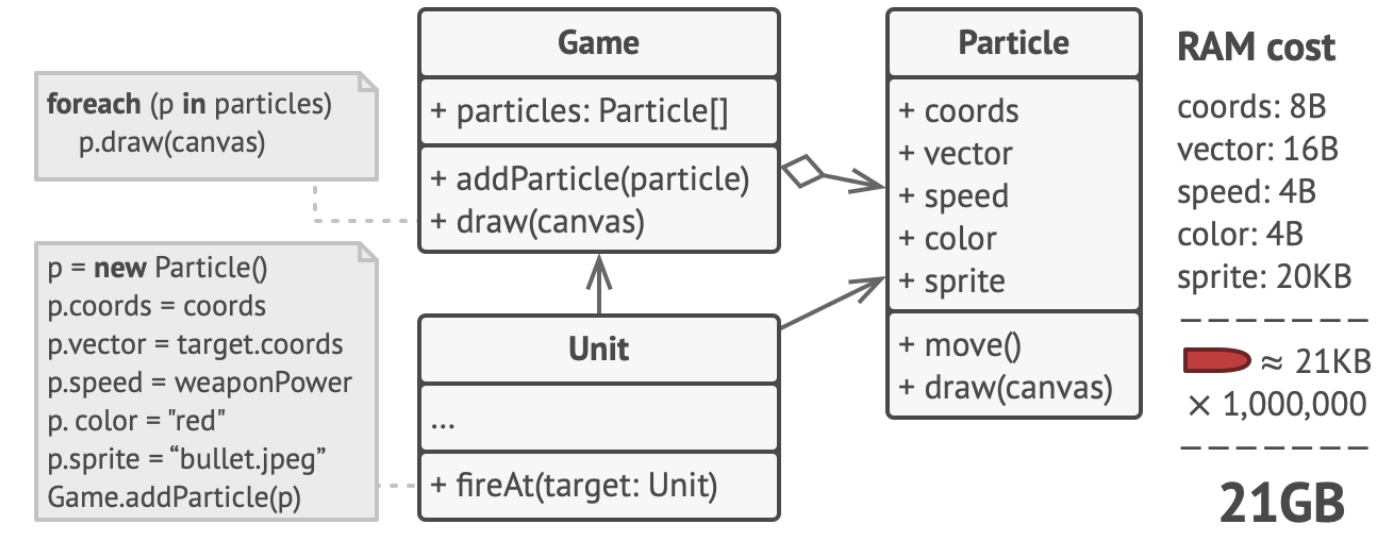
\includegraphics[width=1\linewidth]{assets/pattern/flyweight/flyweight-problema.png}
    \caption{Problema del particle system}
\end{figure}

\paragraph{Problema} Si consideri ad esempio un semplice videogioco in cui si è scelto di implementare un sistema particellare realistico e renderlo una caratteristica distintiva. Grandi quantità di proiettili, missili e schegge di esplosioni dovrebbero volare su tutta la mappa di gioco. Ogni particella è rappresentata da un oggetto separato contenente molti dati. Durante l’esecuzione, ad un certo punto, non c'è più spazio a sufficienza nella RAM per le particelle appena create, quindi il programma va in crash.

\begin{figure}[H]
    \centering
    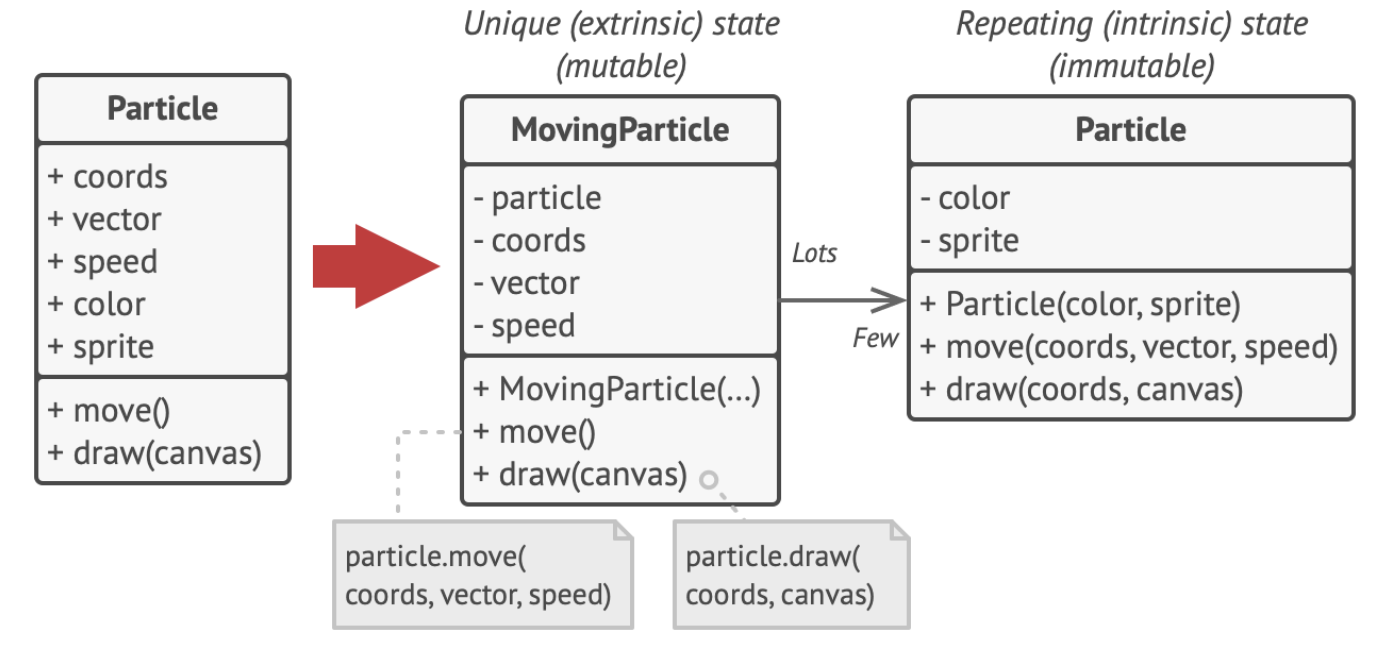
\includegraphics[width=1\linewidth]{assets/pattern/flyweight/flyweight-soluzione.png}
    \caption{Soluzione tramite pattern Flyweight}
\end{figure}

\paragraph{Soluzione} Il pattern Flyweight descrive come condividere oggetti in modo da consentire il loro uso a granularità fine senza avere costi proibitivi. Si costruisce un oggetto condiviso che può essere usato simultaneamente in più contesti. Data la loro natura c'è bisogno di distinguere tra stato interno (o intrinseco, informazioni indipendenti dal contesto) e stato esterno (o estrinseco, informazioni dipendenti dal contesto). Lo stato esterno viene passato dal client.

\begin{minipage}{0.5\linewidth}
    \paragraph{Esempio} Nell’esempio i campi color e sprite consumano molta più memoria rispetto agli altri. Inoltre essi memorizzano informazioni pressoché identiche tra le particelle. Ad esempio tutti i proiettili avranno lo stesso colore e lo stesso sprite. Gli altri campi, quali le coordinate, il vettore direzione e la velocità hanno valori distinti per ogni particella e inoltre cambiano con il tempo. Colore e sprite corrispondono allo stato intrinseco mentre gli altri campi allo stato estrinseco. La classe Particle modella lo stato intrinseco (immutabile), la classe MovingParticle quello estrinseco. Solo tre oggetti diversi saranno sufficienti a rappresentare lo stato esterno di tutte le particelle del gioco: uno per i proiettili, uno per il missili e uno per le schegge. Nell’esempio lo stato intrinseco è memorizzato nell’array particle della classe Game mentre quello estrinseco nell’array mps. Una soluzione più elegante consiste nell’introdurre una classe di contesto che memorizza lo stato estrinseco e un riferimento all’oggetto flyweight che corrisponde a quello intrinseco.
\end{minipage}
\hfill
\begin{minipage}{0.5\linewidth}
    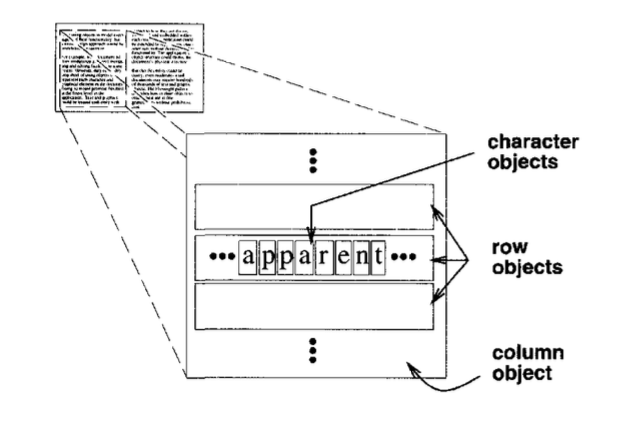
\includegraphics[width=1\linewidth]{assets/pattern/flyweight/flyweight-esempio.png}
\end{minipage}

\begin{figure}[H]
    \centering
    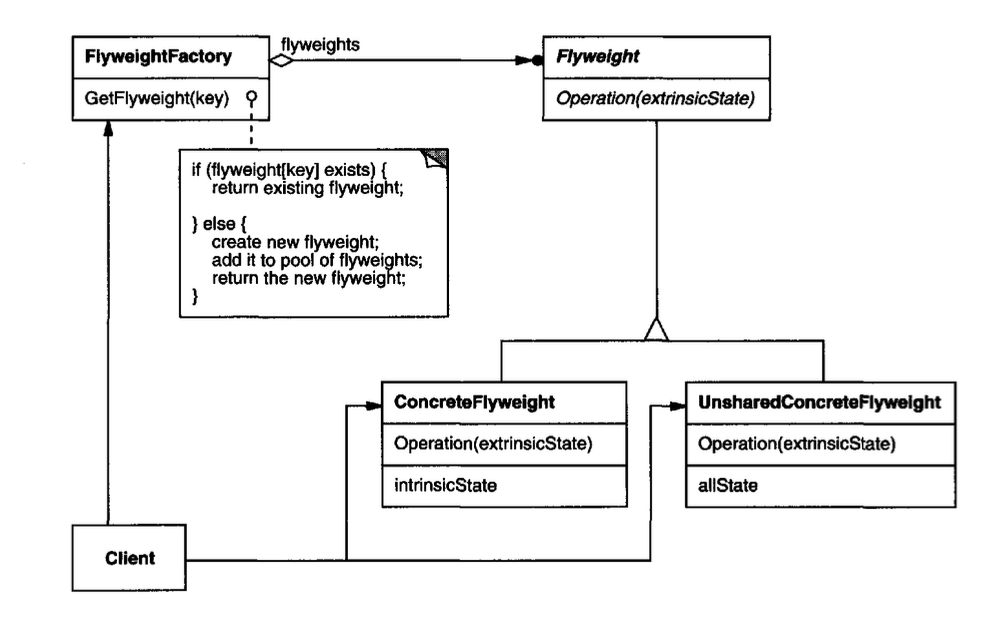
\includegraphics[width=1\linewidth]{assets/pattern/flyweight/flyweight-struttura.png}
    \caption{Class Diagram del pattern Flyweight}
\end{figure}

\paragraph{Struttura e Conseguenze} Il pattern è composto da:
\begin{itemize}
    \item \textbf{Flyweight}: dichiara un’interfaccia attraverso la quale gli oggetti flyweight possono ricevere lo stato esterno e agire di conseguenza.
    \item \textbf{FlyweightFactory}: crea e gestisce gli oggetti flyweight. Si assicura che i flyweight siano condivisi in modo appropriato. Quando un client richiede un flyweight, l’oggetto FlyweightFactory restituisce un’istanza esistente, oppure, se non esiste alcuna istanza, prima la crea e poi la restituisce.
    \item \textbf{Context}: contiene lo stato estrinseco, unico tra tutti gli oggetti originali. Quando un oggetto context è accoppiato con uno degli oggetti flyweight, rappresenta l’intero stato di un oggetto originale.
    \item \textbf{Client}: calcola oppure memorizza lo stato estrinseco dei flyweight. Dal punto di vista del client, un flyweight è un oggetto template che può essere configurato a tempo di esecuzione fornendogli dati contestuali come parametri dei suoi metodi.
\end{itemize}

\newpage
\subsection{Proxy}

\textbf{Scopo}: Strutturale \\
\textbf{Raggio d'azione}: Oggetti

\paragraph{Definizione} Fornisce un surrogato o segnaposto di un altro oggetto per controllare l'accesso a tale oggetto.

\paragraph{Problema} Si consideri un editor che consente di rappresentare anche immagini all’interno dei documenti. Per velocizzare il caricamento in memoria dei documenti può essere opportuno ritardare il caricamento delle immagini fino a quando non è necessario visualizzarle.

\paragraph{Soluzione} Utilizzare un oggetto surrogato dell’immagine, ad esempio che occupi lo stesso spazio

\begin{figure}[H]
    \centering
    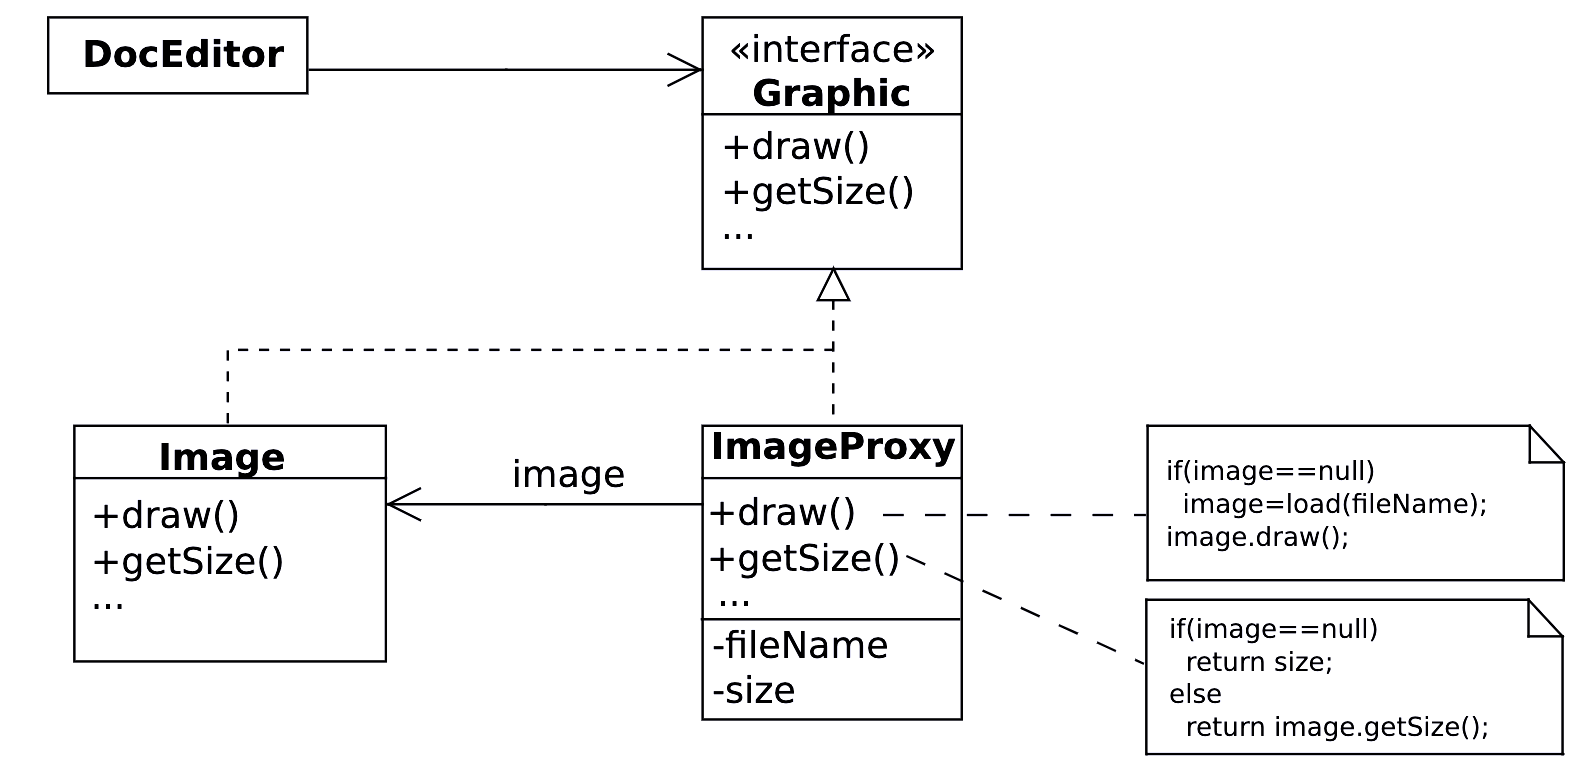
\includegraphics[width=1\linewidth]{assets/pattern/proxy/proxy-esempio.png}
    \caption{Esempio di utilizzo del pattern}
\end{figure}

\paragraph{Struttura e Conseguenze} Il pattern è composto da:
\begin{itemize}
    \item \textbf{Proxy} (ImageProxy): mantiene un riferimento all'oggetto di tipo RealSubject (di cui è \textit{surrogato}). Ha la stessa interfaccia di Subject. Controlla l'accesso all'oggetto rappresentato e può essere responsabile della sua creazione o eliminazione;
    \item \textbf{Subject} (Graphic): definisce l'interfaccia comune per RealSubject e Proxy consentendo di usare Proxy ove ci si attende un RealSubject
    \item \textbf{RealSubject} (Image): definisce l'oggetto reale rappresentato dal proxy;
\end{itemize}


\begin{figure}[H]
    \centering
    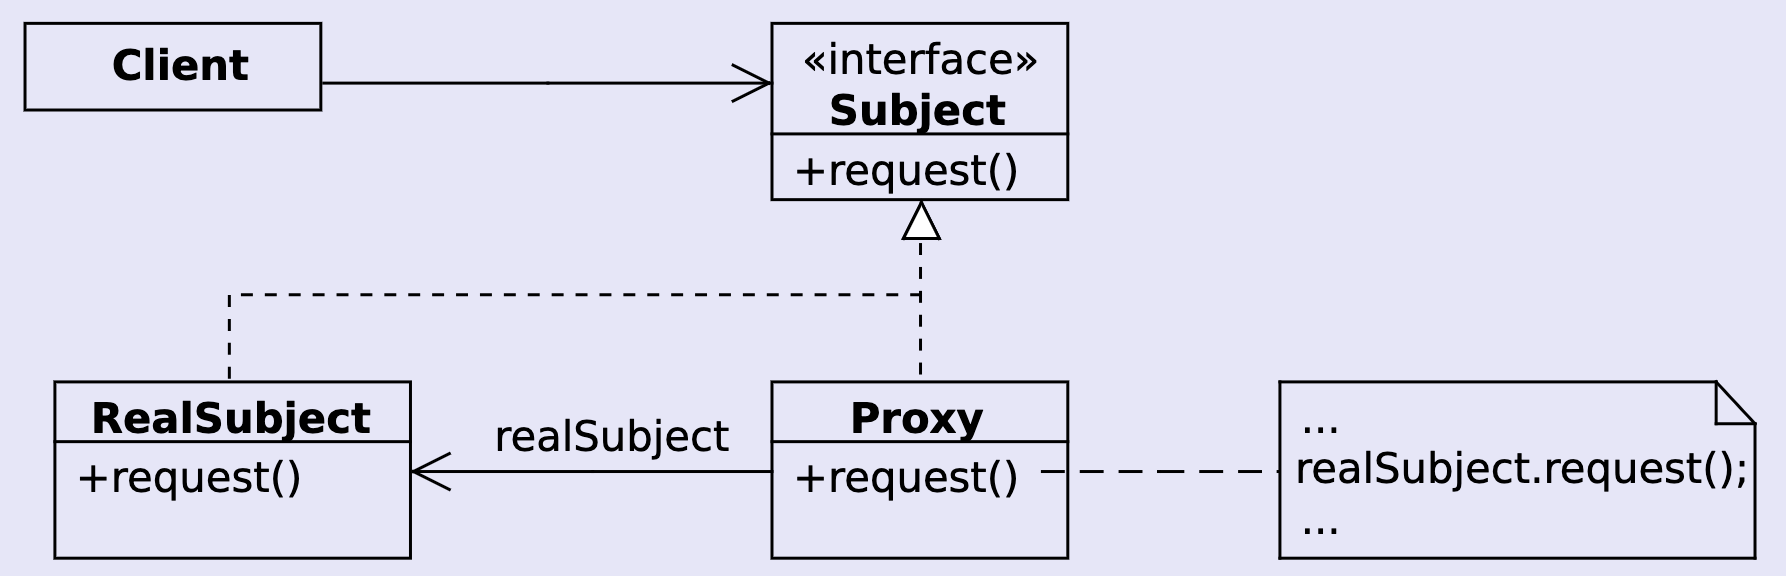
\includegraphics[width=1\linewidth]{assets/pattern/proxy/proxy-struttura.png}
    \caption{Struttura del pattern}
\end{figure}

\textbf{Esempio Java}
\begin{minted}[
    fontsize=\footnotesize,
    linenos,
]{java}
// Proxy implements Subject
public class ListaSicura<E> implements Lista<E> {

    private Lista<E> lista;
    private PermessiUtente pu; // RealSubject

    public ListaSicura(Lista<E> l, int nread, int nwrite) {
        lista = l;
        pu = new PermessiUtente(nread, nwrite);
    }

    @Override
    public void aggiungi(int index, E dato) throws IndexOutOfBoundsException {
        if(pu.getNumeroScritture() == 0) {
            throw new AccessoNonConsentitoException
        }
        pu.decrementaScritture();
        lista.aggiungi(index, dato);
    }

}
\end{minted}


\newpage

\section{Comportamentali}

I pattern comportamentali permettono di 
\begin{itemize}
    \item \textbf{Class Behavioral}: Utilizzare l'ereditarietà per distribuire il comportamento tra le classi.
    \item \textbf{Object Behavioral}: Utilizzare la composizione degli oggetti piuttosto che l'ereditarietà (per distribuire il comportamento tra le classi).
\end{itemize}

\subsection{Chain of Responsability}
\label{chain-of-responsability}

\textbf{Scopo}: Comportamentale \\
\textbf{Raggio d'azione}: Oggetti

\paragraph{Definizione} Il pattern Chain of Responsability permette di evitare l'accoppiamento di una richiesta del mittente e del destinatario, facendo in modo che entrambi riescano ad averla esaudita. Consente di passare le richieste lungo una catena di gestori. Dopo aver ricevuto una richiesta, ciascun gestore decide di elaborarla o di trasmetterla al gestore successivo nella catena.

\begin{figure}[H]
    \centering
    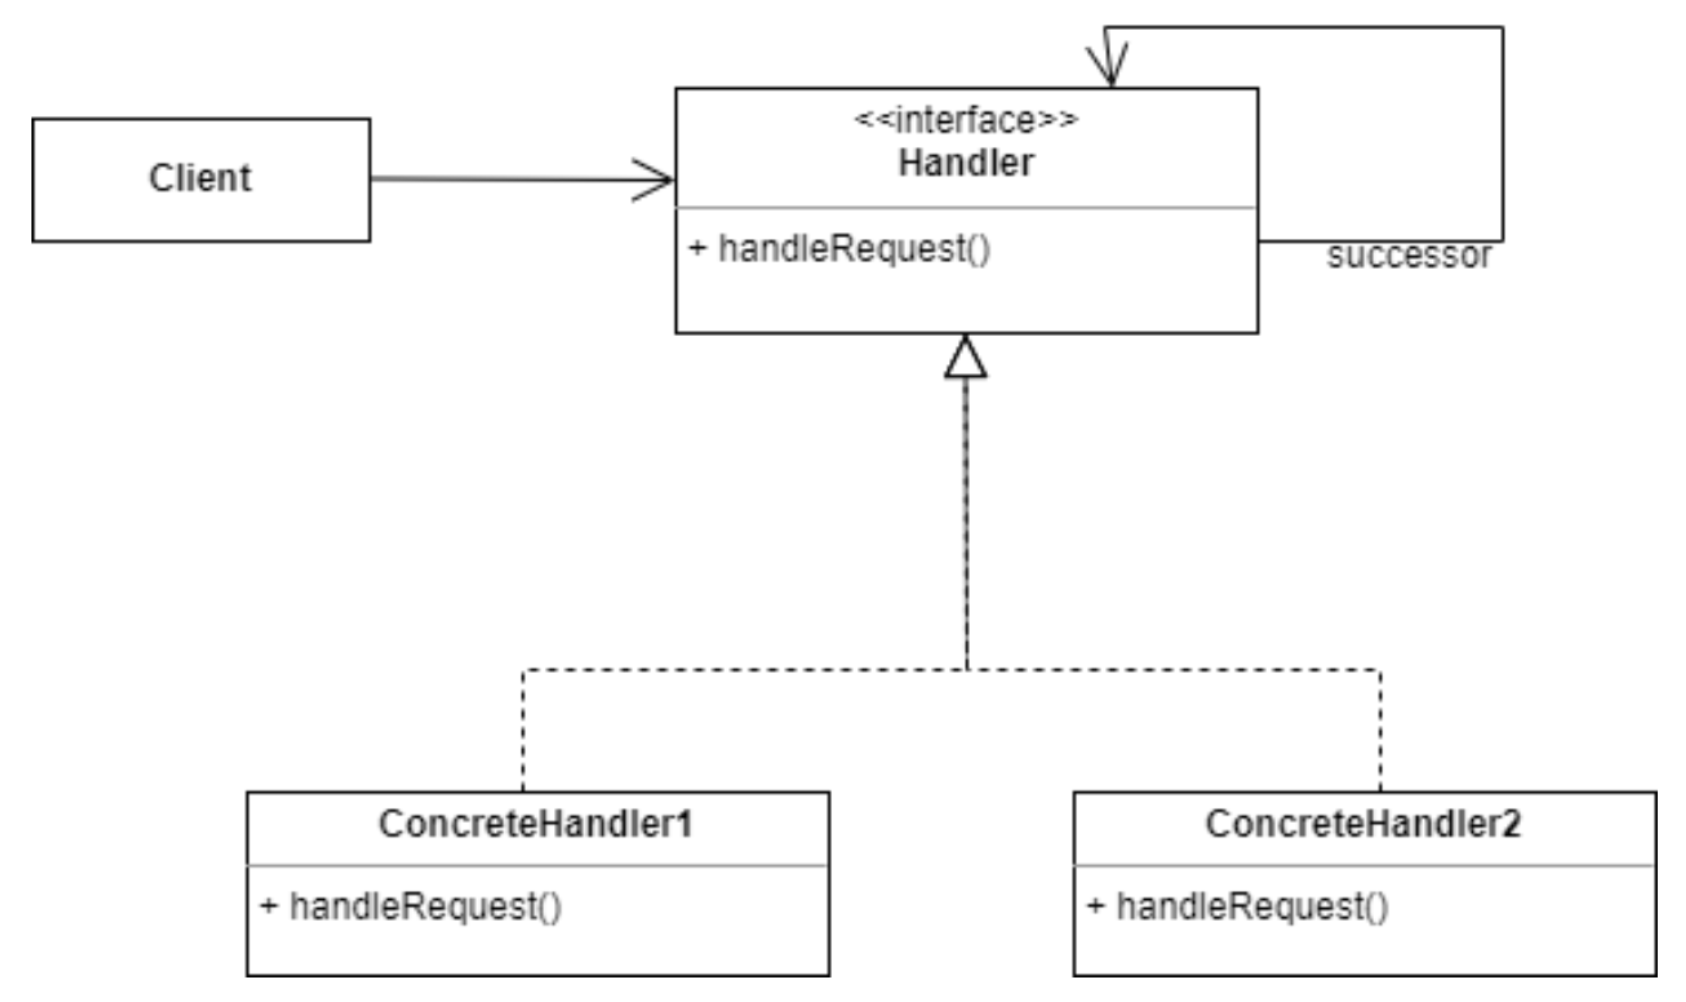
\includegraphics[width=0.4\linewidth]{assets/pattern/chain-of-responsability/cor-struttura.png}
    \caption{Struttura del pattern}
\end{figure}

\paragraph{Applicabilità} Il pattern CoR risulta utile quando si prevede che il programma elabori diversi tipi di richieste in vari modi, ma i tipi esatti di richieste e le relative sequenze sono sconosciuti in anticipo, quando è essenziale eseguire diversi gestori in un ordine particolare o quando si suppone che l'insieme di gestori e il relativo ordine cambino in fase di esecuzione.

CoR viene spesso utilizzata insieme a Composite (\ref{composite}). In questo caso, quando un componente foglia riceve una richiesta, può passarla attraverso la catena di tutti i componenti genitore fino alla radice dell'albero degli oggetti.

\begin{figure}[H]
    \centering
    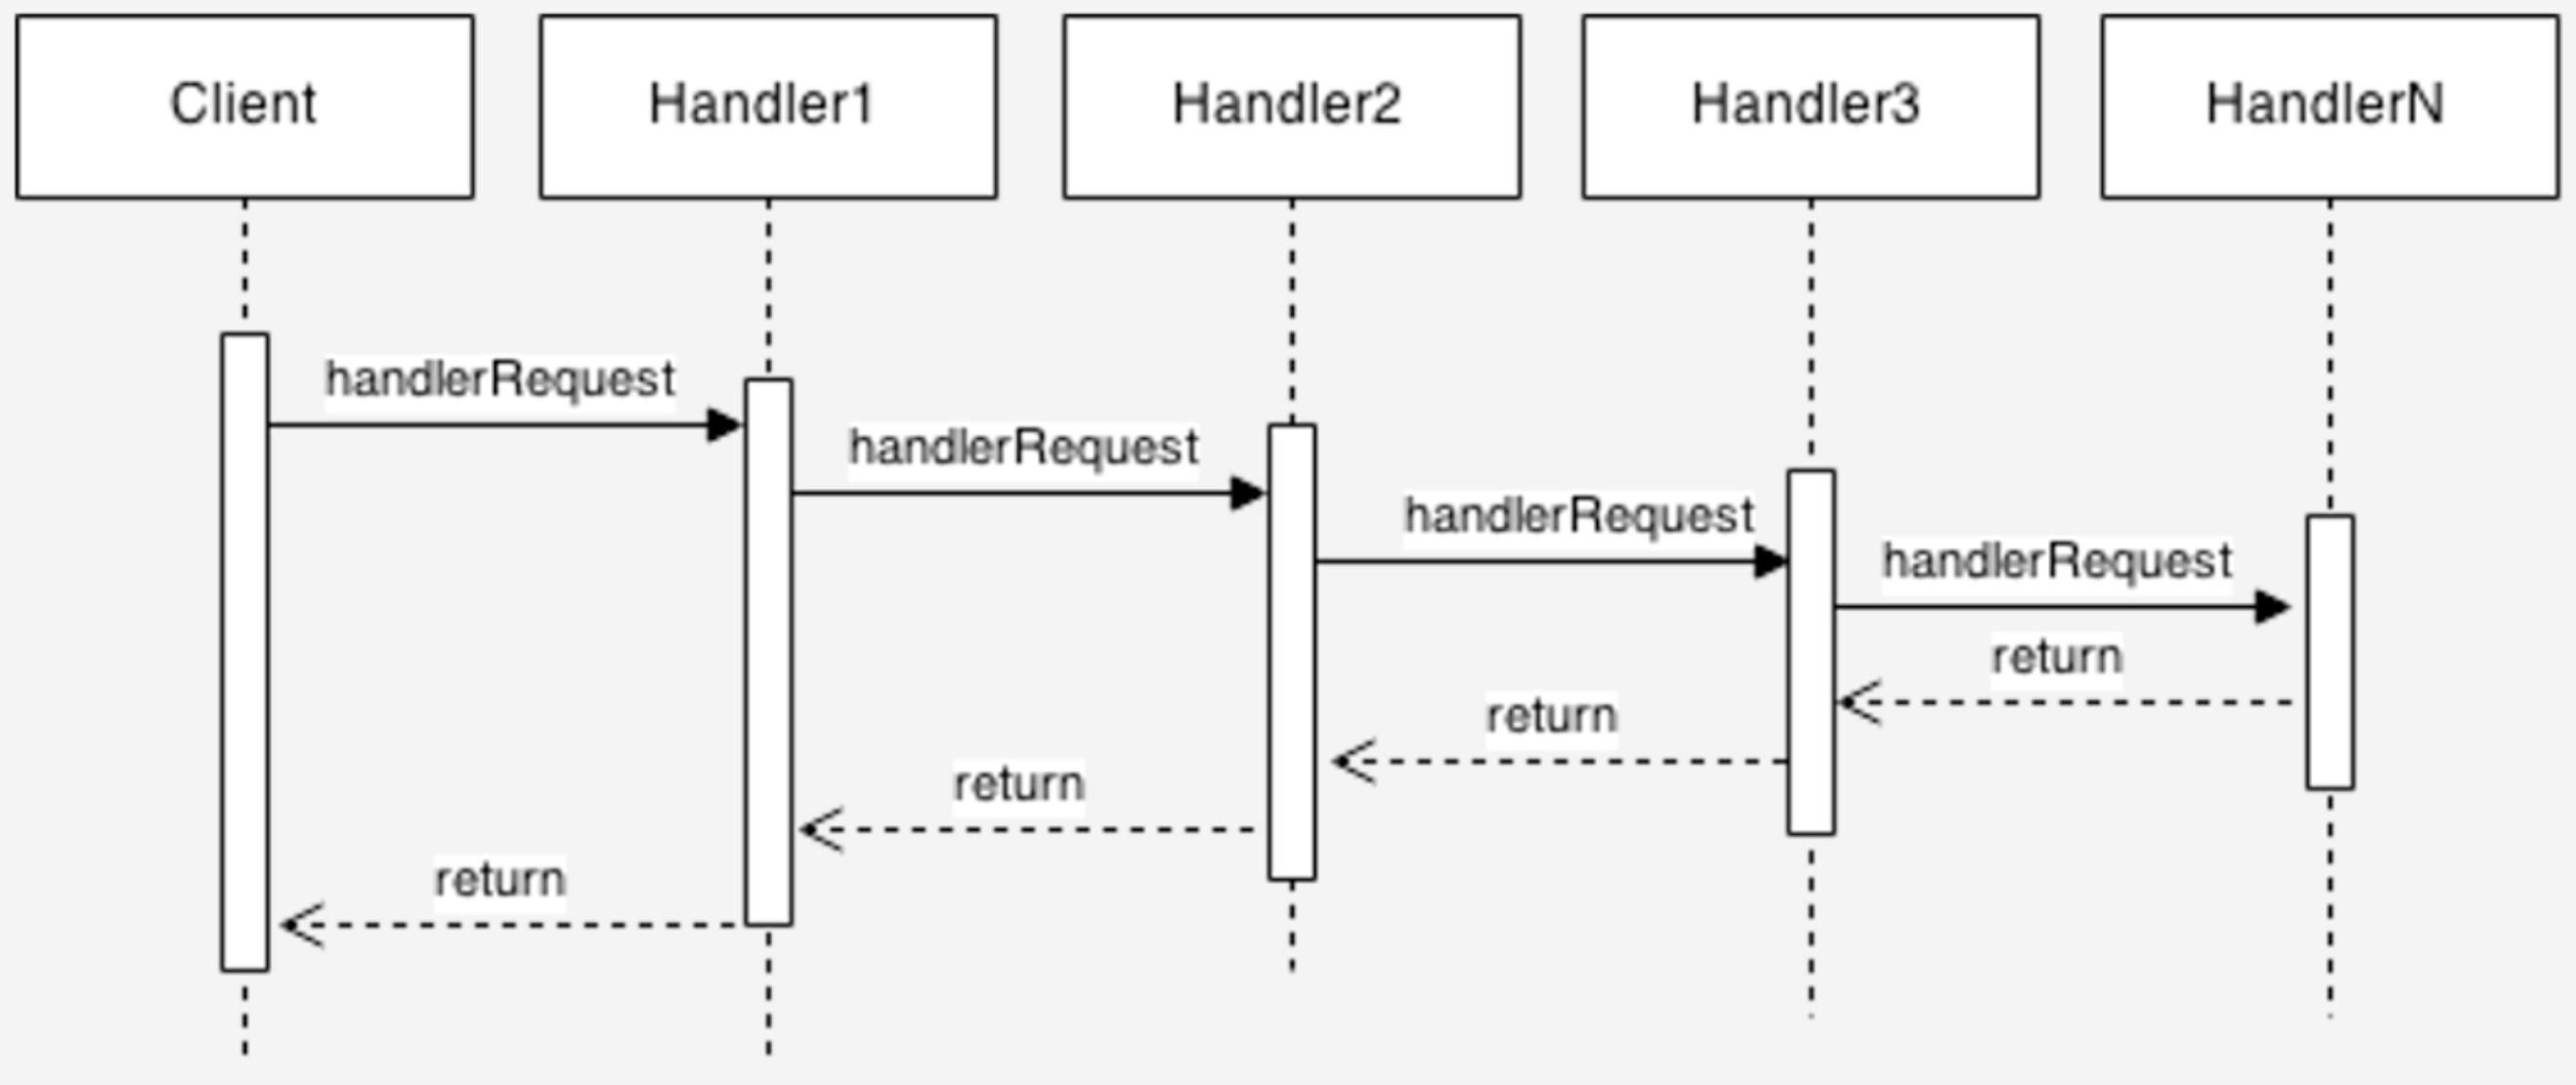
\includegraphics[width=0.8\linewidth]{assets/pattern/chain-of-responsability/cor-sequence.png}
    \caption{Sequence Diagram del patter Chain of Responsability}
\end{figure}

\newpage
\subsection{Command}
\label{command}

\textbf{Scopo}:  \\
\textbf{Raggio d'azione}: 

\paragraph{Definizione}

\paragraph{Problema}

\paragraph{Soluzione} 

\paragraph{Struttura e Conseguenze} 

\newpage
\subsection{Interpreter}
\label{interpreter}

\textbf{Scopo}: Comportamentale \\
\textbf{Raggio d'azione}: Oggetti

\paragraph{Definizione} Modello di progettazione che, dato un linguaggio, permette di definire una rappresentazione della sua grammatica insieme a un interprete che utilizza tale rappresentazione per interpretare le frasi in quel linguaggio.

Si definiscono classi di espressioni terminali (elementi di base) e non terminali (combinazioni di elementi), organizzate in una struttura ad albero simile al pattern Composite (\ref{composite}).

\paragraph{Motivazione} Se un particolare tipo di problema si presenta abbastanza frequentemente, allora potrebbe essere utile esprimere le istanze del problema come frasi in un linguaggio semplice, costruendo poi un interprete che risolve il problema interpretando queste frasi. Per esempio, la ricerca di stringhe che corrispondono a un pattern è un problema comune, e le espressioni regolari sono un linguaggio standard per specificare pattern di stringhe: piuttosto che costruire algoritmi personalizzati per far corrispondere ogni pattern alle stringhe, gli algoritmi di ricerca potrebbero interpretare un'espressione regolare che specifica un insieme di stringhe da far corrispondere.

\begin{multicols}{2}
    \begin{figure}[H]
        \centering
        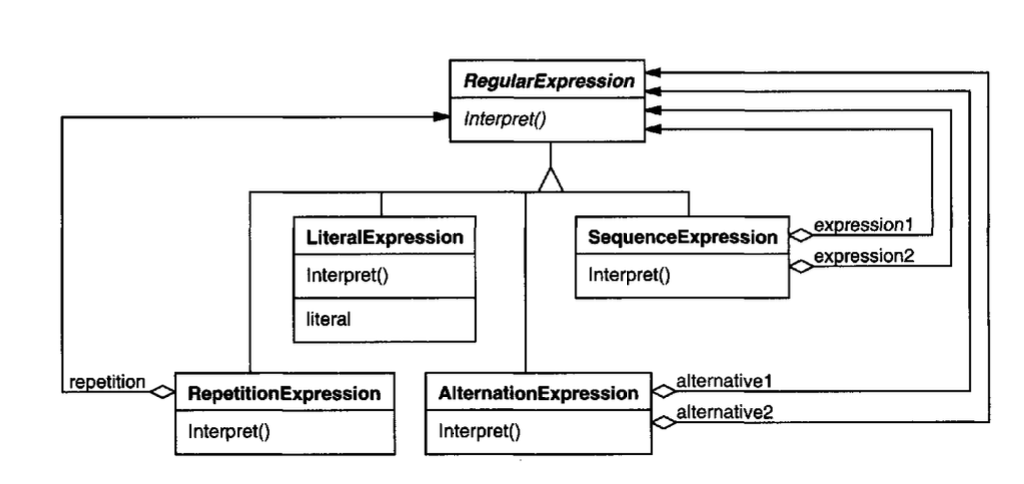
\includegraphics[width=1\linewidth]{assets/pattern/interpreter/interpreter-esempio-class.png}
    \end{figure}
    \columnbreak
    \begin{figure}[H]
        \centering
        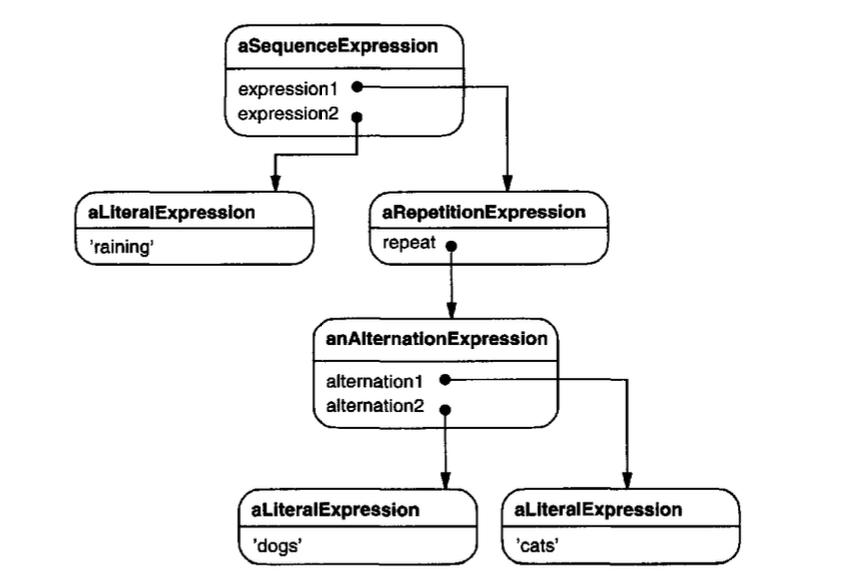
\includegraphics[width=1\linewidth]{assets/pattern/interpreter/interpreter-esempio-object.png}
    \end{figure}
\end{multicols}

Il pattern Interpreter descrive come definire una grammatica per linguaggi semplici, rappresentare frasi nel linguaggio e interpretare queste frasi, usando nel nostro esempio una classe per rappresentare ogni regola grammaticale dove i simboli sul lato destro della regola sono variabili di istanza di queste classi. Ogni espressione regolare definita dalla grammatica è rappresentata da un albero sintattico astratto composto da istanze di queste classi, e possiamo creare un interprete per queste espressioni regolari definendo l'operazione Interpret su ogni sottoclasse che prende come argomento il contesto in cui interpretare l'espressione, contenente la stringa di input e informazioni su quanto di essa è già stata fatta corrispondere. Ogni sottoclasse implementa Interpret per far corrispondere la parte successiva della stringa di input basandosi sul contesto corrente: LiteralExpression controllerà se l'input corrisponde al letterale che definisce, AlternationExpression controllerà se l'input corrisponde a una qualsiasi delle sue alternative, RepetitionExpression controllerà se l'input ha copie multiple dell'espressione che ripete, e così via.

\newpage

\paragraph{Applicabilità} È consigliabile utilizzare il pattern Interpreter quando:
\begin{itemize}
    \item Dato un linguaggio da interpretare, si vogliono rappresentare le sue istruzioni come alberi sintattici astratti;
    \item La grammatica del linguaggio è relativamente semplice;
    \item L'efficienza non è una preoccupazione fondamentale;
\end{itemize}

\begin{figure}[H]
    \centering
    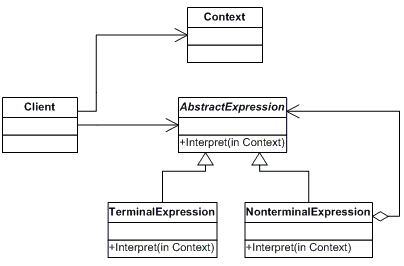
\includegraphics[width=0.75\linewidth]{assets/pattern/interpreter/interpreter-struttura.png}
    \caption{Class Diagram del pattern Interpreter}
\end{figure}

\paragraph{Struttura} Il pattern comprende:
\begin{itemize}
    \item \textbf{AbstractExpression}: Interfaccia o classe astratta che dichiara il metodo \texttt{interpreta}, comune a tutte le espressioni.
    \item \textbf{TerminalExpression}: Classi concrete che rappresentano i simboli di base della grammatica (foglie dell'albero), come numeri o variabili.
    \item \textbf{NonterminalExpression}: Classi concrete che rappresentano combinazioni di espressioni e gestiscono la logica di interpretazione delle sottoespressioni.
    \item \textbf{Context}: contiene informazioni globali per l'interprete.
    \item \textbf{Client}: costruisce (o riceve) un albero sintattico astratto che rappresenta una particolare frase nella lingua definita dalla grammatica. L'albero sintattico astratto è assemblato da istanze delle classi NonterminalExpression e TerminalExpression. Richiama l'operazione \textit{Interpret()}.
\end{itemize}

Le espressioni non terminali coordinano l'interpretazione delle sottoespressioni, aggregando i risultati per ottenere il valore finale dell'espressione.


\paragraph{Conseguenze} Il pattern Interpreter consente quindi di:
\begin{itemize}
    \item Facilitare la modifica ed estensione della grammatica di un dato linguaggio;
    \item Aggiungere nuovi modi per interpretare le espressioni;
\end{itemize}

È bene notare che le grammatiche complesse sono difficili da mantenere.

\newpage

\subsection{Iterator}
\label{iterator}

\textbf{Scopo}:  \\
\textbf{Raggio d'azione}: 

\paragraph{Definizione}

\paragraph{Problema}

\paragraph{Soluzione} 

\paragraph{Struttura e Conseguenze} 

\newpage
\subsection{Mediator}


\textbf{Scopo}:  \\
\textbf{Raggio d'azione}: 

\paragraph{Definizione}

\paragraph{Problema}

\paragraph{Soluzione} 

\paragraph{Struttura e Conseguenze} 

\newpage
\subsection{Memento}
\label{memento}

\textbf{Scopo}:  \\
\textbf{Raggio d'azione}: 

\paragraph{Definizione}

\paragraph{Problema}

\paragraph{Soluzione} 

\paragraph{Struttura e Conseguenze} 

\newpage
\subsection{Observer (\textit{o Dependents, Publish-Subscribe})}
\label{observer}

\textbf{Scopo}: Comportamentale \\
\textbf{Raggio d'azione}: Oggetti

\paragraph{Definizione} Il pattern Observer permette di definire una dipendenza uno a molti tra oggetti, in modo tale che se un oggetto cambia il suo stato, tutti gli oggetti dipendenti da questo siano notificati e aggiornati automaticamente.

\begin{figure}[H]
    \centering
    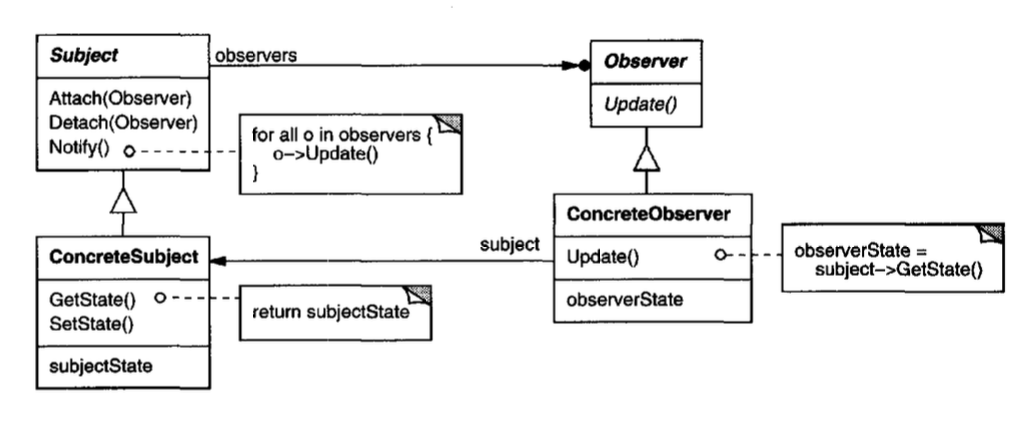
\includegraphics[width=1\linewidth]{assets/pattern/observer/observer-struttura.png}
    \caption{Class Diagram del pattern Observer}
\end{figure}

\paragraph{Struttura} Il pattern è composto da:
\begin{itemize}
    \item \textbf{Subject}: conosce i propri osservatori; un numero qualunque di oggetti Observer può osservare un soggetto. Fornisce un’interfaccia per registrare e cancellare le registrazioni degli oggetti Observer. 
    \item \textbf{Observer}: fornisce un’interfaccia di notifica per gli oggetti a cui devono essere notificati i cambiamenti nel Subject. 
    \item \textbf{ConcreteSubject}: contiene lo stato a cui gli oggetti 
     ConcreteObserver sono interessati. Inoltra una notifica ai suoi Observer quando il proprio stato si modifica. 
    \item \textbf{ConcreteObserver}: memorizza un riferimento a un oggetto ConcreteSubject oppure ottiene dinamicamente il riferimento all’oggetto Subject da cui ha origine la notifica in caso in esso cui osservi più Subject. Contiene informazioni che devono essere sincronizzate con lo/gli stato/i del/i Subject. Implementa l’interfaccia Observer per ricevere le notifiche del Subject.
\end{itemize}

\begin{figure}[H]
    \centering
    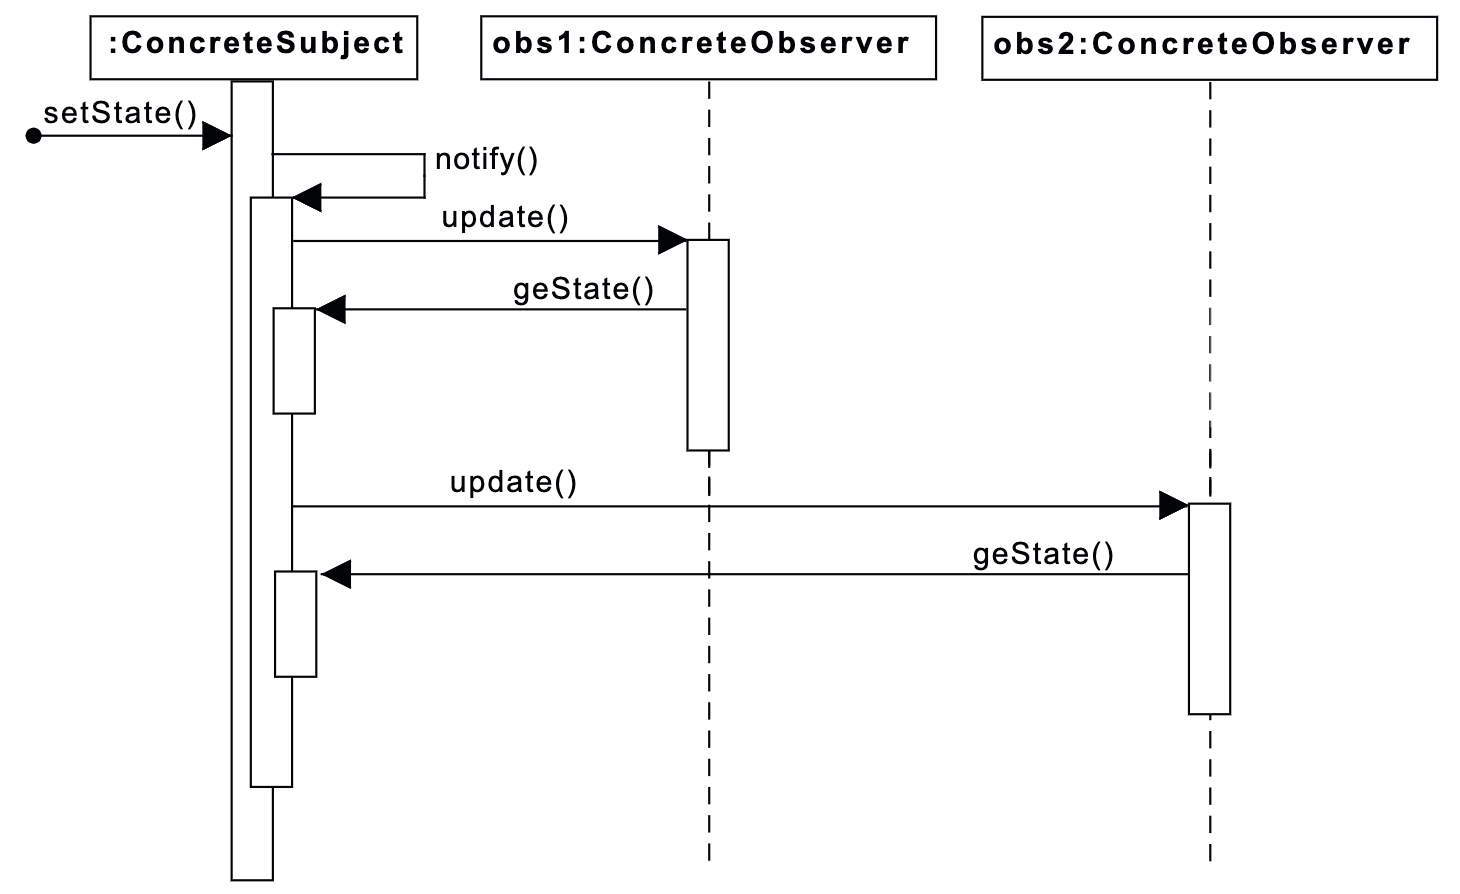
\includegraphics[width=1\linewidth]{assets/pattern/observer/observer-sequence.png}
    \caption{Sequence Diagram del pattern Observer}
\end{figure}

\paragraph{Interazioni} ConcreteSubject notifica i propri Observer quando avviene un cambiamento che potrebbe rendere il loro stato non inconsistente rispetto al proprio. Dopo essere stato informato di un cambiamento nel ConcreteSubject, un osservatore concreto può chiedere al Subject informazioni sul suo stato. ConcreteObserver usa questa informazione per riconciliare il suo stato con quello del subject.

\newpage
\subsection{State}
\label{state}

\textbf{Scopo}:  \\
\textbf{Raggio d'azione}: 

\paragraph{Definizione}

\paragraph{Problema}

\paragraph{Soluzione} 

\paragraph{Struttura e Conseguenze} 

\newpage
\subsection{Strategy}


\textbf{Scopo}:  \\
\textbf{Raggio d'azione}: 

\paragraph{Definizione}

\paragraph{Problema}

\paragraph{Soluzione} 

\paragraph{Struttura e Conseguenze} 

\newpage
\subsection{Template Method}
\label{template-method}

\textbf{Scopo}: Comportamentale \\
\textbf{Raggio d'azione}: Classi

\paragraph{Definizione} Il pattern definisce la struttura di un algoritmo all'interno di un metodo, delegando alcuni passi alle sottoclassi (motivo per cui è un pattern class-based).

Consente, introducendo sottoclassi diverse, di cambaire il modo in cui i sottopassi vengono eseguiti, lasciando inalterata la struttura dell'algoritmo che è stato inglobato.

\paragraph{Motivazione} Considera un framework applicativo che fornisce classi Application e Document, dove la classe Application è responsabile di aprire documenti esistenti memorizzati in un formato esterno come un file, e un oggetto Document rappresenta le informazioni in un documento una volta che è stato letto dal file. Le applicazioni costruite con il framework possono creare sottoclassi di Application e Document per soddisfare bisogni specifici: per esempio, un'applicazione di disegno definisce sottoclassi DrawApplication e DrawDocument, mentre un'applicazione foglio di calcolo definisce sottoclassi SpreadsheetApplication e SpreadsheetDocument. La classe astratta Application definisce l'algoritmo per aprire e leggere un documento nella sua operazione OpenDocument che definisce ogni passo per aprire un documento: controlla se il documento può essere aperto, crea l'oggetto Document specifico dell'applicazione, lo aggiunge al suo insieme di documenti, e legge il Document da un file. Chiamiamo OpenDocument un template method, che definisce un algoritmo in termini di operazioni astratte che le sottoclassi sovrascrivono per fornire comportamento concreto, dove le sottoclassi Application definiscono i passi dell'algoritmo che controllano se il documento può essere aperto (CanOpenDocument) e che creano il Document (DoCreateDocument), mentre le classi Document definiscono il passo che legge il documento (DoRead).

\begin{figure}[H]
    \centering
    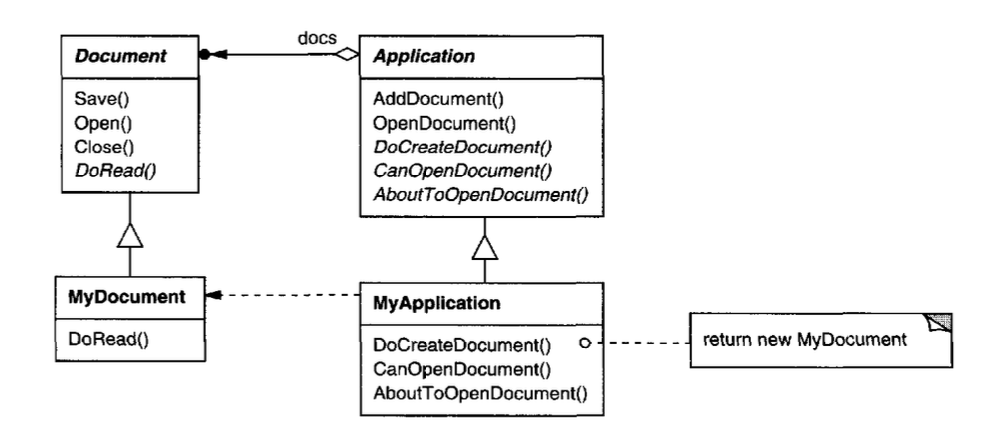
\includegraphics[width=0.75\linewidth]{assets/pattern/template-method/template-esempio.png}
\end{figure}

Il template method definisce anche un'operazione che permette alle sottoclassi Application di sapere quando il documento sta per essere aperto (AboutToOpenDocument), nel caso sia di loro interesse. Definendo alcuni dei passi di un algoritmo usando operazioni astratte, il template method fissa il loro ordine, ma permette alle sottoclassi Application e Document di variare quei passi per soddisfare i loro bisogni.

\paragraph{Applicabilità} Il pattern Template Method è utile quando:
\begin{itemize}
    \item Si desidera implementare una volta sola le parti invarianti di un algoritmo e lasciare alle sottoclassi l'implementazione dei comportamenti che possono variare.
    \item I comportamenti comuni tra le sottoclassi devono essere fattorizzati e localizzati in una classe comune per evitare la duplicazione del codice;
    \item Si vogliono controllare le estensioni delle sottoclassi;
\end{itemize}

\begin{figure}[H]
    \centering
    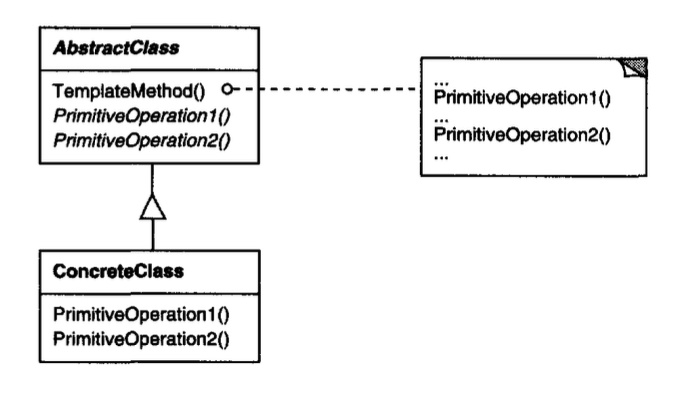
\includegraphics[width=0.5\linewidth]{assets/pattern/template-method/template-struttura.png}
    \caption{Class Diagram del pattern Template}
\end{figure}

\paragraph{Struttura} Il pattern è composto da:
\begin{itemize}
    \item \textbf{AbstractClass} (Applicazione): definisce operazioni primitive astratte che le sottoclassi concrete definiscono per implementare le fasi di un algoritmo.Implementa un metodo modello che definisce lo scheletro di un algoritmo. Il metodo modello richiama operazioni primitive, operazioni definite in AbstractClass o quelle di altri oggetti.
    \item \textbf{ConcreteClass} (MyApplication): implementa le operazioni primitive per eseguire le fasi dell'algoritmo specifiche della sottoclasse.
\end{itemize}

ConcreteClass si basa su AbstractClass per implementare i passaggi invarianti dell'algoritmo.

\begin{figure}[H]
    \centering
    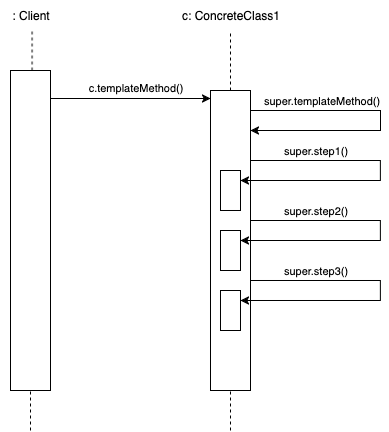
\includegraphics[width=0.5\linewidth]{assets/pattern/template-method/template-sequence.drawio.png}
    \caption{Sequence Diagram del pattern Template}
\end{figure}

\paragraph{Conseguenze} Il pattern Template Method consente quindi di:
\begin{itemize}
    \item Riutilizzare codice già scritto;
    \item Applicare il \textbf{principio di Hollywood} (Don't call us, we'll call you): la classe padre chiama le operazioni di una sottoclasse e non viceversa;
\end{itemize}

Il pattern permette di rimuovere codice duplicato inserendolo nella AbstractClass, però alcuni client potrebbero essere limitati dallo scheletro fornito di un dato algoritmo. In più i metodi tendono ad essere più difficili da mantenere all'aumentare dei passaggi forniti.



\newpage
\subsection{Visitor}


\textbf{Scopo}:  \\
\textbf{Raggio d'azione}: 

\paragraph{Definizione}

\paragraph{Problema}

\paragraph{Soluzione} 

\paragraph{Struttura e Conseguenze} 

\newpage